%%%%%%%%%%%%%%%%%%%%%%%%%%%%%%%%%%%%%%%%%%%%%%%%
% Plantilla para la Elaboración de Tesis
% Universidad Nacional de Misiones - Argentina
% Realizado por: Carlos Brys
% Contacto: carlos.brys@fce.unam.edu.ar /       Telegram:@CarlosBrys
%%%%%%%%%%%%%%%%%%%%%%%%%%%%%%%%%%%%%%%%%%%%%%%%

%!TEX root = 1_Tesis.tex

\RequirePackage{etex}

\documentclass[
titlepage,
oneside,
openright,
onecolumn,
a4paper,
12pt]{book}

% Text encoding to take for data input stream. I.e. the text we write in.
% How to encode fonts.
%\usepackage[T1]{fontenc}
%usepackage{ucs}              %% Unicode support
%\usepackage[T1]{fontenc}
\usepackage[utf8]{inputenc}
\usepackage{amsmath}
\usepackage{epigraph}

% Para mostrar el icono ORCID
\usepackage{academicons}
\usepackage{fontawesome5}
\usepackage{etoolbox}

% Leave the smallest margins on A4 paper.
\usepackage{a4wide}

% Configuracion de los margenes de la pagina
% Ver: https://es.sharelatex.com/learn/Page_size_and_margins
\usepackage{geometry}
\geometry{
 a4paper,
 left=3.5cm, right=2.0cm,
 top=2.5cm, bottom=2.5cm}

% Separacion entre párrafos
%\setlength\parskip{\medskipamount}
\setlength\parskip{\bigskipamount}

% Separacion en las listas
\usepackage{enumitem}
\setlist{noitemsep} % Uncomment this if you want it as a global setting

% Sangría en la primera línea
\setlength\parindent{50pt}

% Para importar archivos pdf (la portada)
\usepackage{pdfpages} 
\usepackage{pdflscape}

% Para comentar parrafos
\usepackage{comment}

% Tamaño de la fuente del pie de imagen
\usepackage{caption}
\captionsetup{font=footnotesize}
\captionsetup[figure]{name=Figura} % se agrega para cambiar "Ímagen" por "Figura"
% Fancy LaTeX chapter styles
% Options: Sonny, Lenny, Glenn, Conny, Rejne, Bjarne, Bjornstrup
\usepackage[Sonny]{fncychap}

\ChNumVar{\fontsize{76}{80}\usefont{OT1}{pzc}{m}{n}\selectfont}
\ChTitleVar{\raggedleft\huge\sffamily\bfseries}  
\ChNameVar{\bfseries\Large\sf}
%\ChNumVar{\Huge}
%\ChTitleVar{\bfseries\Large\rm}
\ChRuleWidth{1pt}
%\ChNameUpperCase
%\ChTitleUpperCase


% Para insertar hipervinculos  %% SI se actvia, no muestra los indices
\usepackage[pageanchor]{hyperref}
%\usepackage{url} Reduntante su see usa hyperref
%\usepackage[anythingbreaks]{breakurl} % Para cortar las URL largas

\hypersetup{
    colorlinks=true,
    linkcolor=blue,
    filecolor=magenta,      
    urlcolor=cyan,
    citecolor=blue,
    pdfpagemode=FullScreen,
    %backref=page,
}
\urlstyle{same}


\usepackage{cleveref}
\usepackage{chngcntr}

% Ver tipografias en: The LaTeX Font Catalogue http://www.tug.dk/FontCatalogue/ 
%% \usepackage{palatino} 
% %\usepackage{tgbonum}
%\usepackage{antpolt}
% %\usepackage{librebaskerville}
% \usepackage{inconsolata}
\usepackage{antpolt}

\usepackage[tight,spanish]{minitoc}

\usepackage[spanish, es-tabla, activeacute]{babel}
\addto\captionsspanish{% se agrega para cambiar "Índice de Imágenes" por "Índice de Figuras"
  \renewcommand{\listfigurename}{Índice de Figuras}%
}

\usepackage{fvextra}
\usepackage{csquotes}

\usepackage[
    backend=biber,
    style=ieee,
    sorting=none
]{biblatex}
\addbibresource{Bibliografia.bib} 

% We need double spacing for the draft, at least. Also required by Univ. PTA.
\usepackage{setspace}
\onehalfspacing
%\doublespacing


% Glosario de términos
%\usepackage{acronym}
%\usepackage[acronym,nopostdot,nogroupskip]{glossaries}
%\usepackage{glossaries}
\usepackage[automake,acronym,nopostdot,nogroupskip]{glossaries-extra}
%\usepackage[version=3]{acro} %list of abbreviations
%\usepackage{acro}[=v3]
%%% Acrónimos %%%
%%%%%%%%%%%%%%%%%%%%

\newacronym{URL}{URL}
{Localizador Uniforme de Recursos (Uniform Resource Locator), una dirección web que especifica la ubicación de un recurso en Internet y el mecanismo para acceder a él}

\newacronym{HTTP}{HTTP}
{Protocolo de Transferencia de Hipertexto (Hypertext Transfer Protocol), utilizado para la comunicación y transferencia de datos en la World Wide Web}

\newacronym{WWW}{WWW}
{World Wide Web, sistema global de información basado en hipertexto que permite acceder y navegar por múltiples recursos en Internet}

\newacronym{P2P}{P2P}
{Red “peer-to-peer” (par a par), un modelo de intercambio directo de recursos entre usuarios sin necesidad de un servidor central}


%%% Definiciones %%%
%%%%%%%%%%%%%%%%%%%%

\newglossaryentry{metadatos}
{
    name = metadatos,
    description = {Datos estructurados que describen, explican y permiten localizar o gestionar recursos de información}
}

\newglossaryentry{compilador}
{
    name = compilador,
    description = {Programa que transforma código fuente escrito por un programador en instrucciones ejecutables por una computadora}
}

\newglossaryentry{plataforma}
{
    name = plataforma,
    description = {Infraestructura tecnológica y sociocultural que integra hardware, software, algoritmos y políticas, mediando prácticas sociales y producciones de contenido}
}

\newglossaryentry{multiplataforma}
{
    name = multiplataforma,
    description = {Software o tecnología capaz de ejecutarse e interoperar en múltiples sistemas operativos o entornos digitales}
}

\newglossaryentry{online}
{
    name = online,
    description = {Estado de conexión a una red digital, generalmente Internet, o actividad realizada a través de ella}
}

\newglossaryentry{twitter}
{
    name = Twitter,
    description = {Servicio de microblogging para la publicación breve y dinámica de mensajes}
}

\newglossaryentry{LaTeX}
{
    name = LaTeX,
    description = {Sistema de preparación de documentos basado en TeX, desarrollado por Leslie Lamport, ampliamente utilizado en el ámbito académico y científico}
}

\makeglossaries
%\makeglossaries[main,acronym]
%\makenoidxglossaries



% Nomenclarura (para las variables)
\usepackage[refpage,noprefix]{nomencl}
\makenomenclature
\usepackage{morewrites}
% see https://texfaq.org/FAQ-noroom
%\usepackage{etex} 
%\reserveinserts{28}

% Apendices
\usepackage[toc,page]{appendix}


\usepackage{multicol}         
\usepackage{ccicons} % Iconos Creative Commons

% Para listar código
\usepackage{color}
\definecolor{bluekeywords}{rgb}{0.13,0.13,1}
\definecolor{greencomments}{rgb}{0,0.5,0}
\definecolor{redstrings}{rgb}{0.9,0,0}

\usepackage{listings}
\lstset{
%language=XML,
showspaces=false,
showtabs=false,
breaklines=true,
showstringspaces=false,
breakatwhitespace=true,
escapeinside={(*@}{@*)},
commentstyle=\color{greencomments},
keywordstyle=\color{bluekeywords}\bfseries,
stringstyle=\color{redstrings},
basicstyle=\scriptsize\ttfamily,
columns=fullflexible
}

\lstdefinelanguage{OSM}
{
	morekeywords={node, id, lat, lon, user, uid, visible, version, changeset, timestamp, tag},
    sensitive=false,
}

% para las tablas
\usepackage{xcolor}
\definecolor{LightGray}{gray}{0.9}
\usepackage{lscape}
\usepackage{booktabs}
\usepackage{multirow}
\usepackage{longtable}
\usepackage{colortbl} % Paquete para agregar color a las celdas

\usepackage{graphicx,amsfonts,psfrag,fancyhdr,layout,appendix}
\usepackage{subfigure}

\usepackage[nottoc,notlot,notlof]{tocbibind}   
\usepackage{xpatch}


\usepackage[subfigure]{tocloft}
% Para agregar puntos en los niveles de la tabla de contenidos
\renewcommand{\cftpartleader}{\cftdotfill{\cftdotsep}} % for parts
\renewcommand{\cftchapleader}{\cftdotfill{\cftdotsep}} % for chapters
\renewcommand{\cftsecleader}{\cftdotfill{\cftdotsep}} % for sections

% Añadir las ecuaciones al índice
%\usepackage{etoolbox}
%\AtBeginDocument{\listofequations}

% para poner titulos a las ecuaciones
%\usepackage{capt-of} % Para usar \captionof

\usepackage{makeidx} 
\usepackage{float}
\usepackage{textcomp}

% Para listar los algoritmos
%\usepackage{algorithm2e}
\usepackage{algorithm}
\usepackage{algpseudocode}
\usepackage{listings}
\usepackage{minted}
\usemintedstyle{colorful}

\usepackage{lettrine}
\usepackage{xstring}

\widowpenalty=100000
\clubpenalty=100000
\raggedbottom
%%%% \hyphenpenalty=10000 (almost) prevents hyphenation
\hyphenpenalty=9000
\tolerance=100

% Para queue aparezcan hasta las subsubsecciones en el índice
%\usepackage{etoc}
%\setcounter{secnumdepth}{4}
%\setcounter{tocdepth}{4}

\usepackage{eqparbox}

\usepackage{tocloft} 
\cftsetindents{figure}{1.5em}{3.2em} % Indentación del índice de figuras (se puede variar)
\cftsetindents{chapter}{0em}{3.2em}
\cftsetindents{section}{1.5em}{3.2em}
\cftsetindents{subsection}{3.0em}{3.2em}
%%%%%%%%%%%%%%%%%%%%%%%%%%%%%%%%%%%%%%%%%%%%%%%%%%%%%
%%Cajas para las ecuaciones
\usepackage{varwidth}
%\usepackage{etoolbox}
\usepackage[most,many,skins,breakable]{tcolorbox}
\usepackage{tikz,lipsum,lmodern}

\newtcolorbox{caja2}[2][]{enhanced, interior hidden, 
coltitle=black, fonttitle=\bfseries\headingfont\large,
attach boxed title to top left={yshift=-2.5mm},
boxed title style={empty, size=small, top=1mm, bottom=2pt},
%boxed title=0.5\linewidth,
frame code={
\path (title.east|-frame.north) coordinate (aux);
\path[draw=blue, fill=blue!5, line width=0.5mm, rounded corners]
(frame.west) |- ([xshift=-2.5mm]title.north east) to[out=0, in=180] ([xshift=7.5mm]aux)-|(frame.east)|-(frame.south)-|cycle;  
},
title={#2},#1}
%%%%%%%%%%%%%%%%%%%%%%%%%%%%%%%%%%%%%%%%%%%%%

\newtcolorbox{caja}[2][]{empty, 
coltitle=black,
fonttitle=\bfseries\sffamily,
attach boxed title to top left={yshift=-2.5mm},
boxed title style={empty, size=small, top=1mm, bottom=0pt},
varwidth boxed title=0.5\linewidth,
frame code={
\path (title.east|-frame.north) coordinate (aux);
\path[draw=black, line width=0.5mm, rounded corners]
(frame.west) |- ([xshift=-2.5mm]title.north east) to[out=0, in=180] ([xshift=7.5mm]aux)-|(frame.east)|-(frame.south)-|cycle;  
},
title={#2},#1}


%%% Definiciones:
\usepackage{tcolorbox}
\tcbuselibrary{theorems}
\newtcbtheorem[number within=section]{definicion}{Definición}%
{colback=black!5!white,colframe=black!75!black,fonttitle=\bfseries}{th}
%%%%%%%%%%%%%%%%%%%%%%%%%%%%%%%%%%


\usepackage{xspace}
\usepackage{morewrites}
 % Carga la configuración general del documento

\begin{document}

\clearpage
\thispagestyle{empty} 
\pagestyle{empty} % no imprimir ni número, ni cabecera ni pié de página

% \includepdf{imagenes/portada.pdf} % Si tiene una imagen de portada
%\clearpage 
%\newpage

\begin{center}

\begin{minipage}{0.45\textwidth}
    \centering
    \includegraphics[width=\linewidth]{imagenes/logo-unam0.png}
\end{minipage}
\hfill
\begin{minipage}{0.35\textwidth}
    \centering
    \includegraphics[width=\linewidth]{imagenes/logo-unam.png}
\end{minipage}

%\hskip 5cm
%\includegraphics[scale=0.2] {imagenes/logo-fce.png}
%\includegraphics[scale=0.2] {imagenes/logo-fhycs.png}

\vspace{1cm}
{\Large\bf Universidad Nacional de Misiones \\}
\vspace{0.4cm}
{\Large\bf Facultad de Ingeniería \\}
\vspace{0.4cm}
{\Huge Tesis de Grado\\}
\vspace{1cm}
{\Huge\bf Gestión del Consumo de Energía en Microrredes Eléctricas \\}
%%{\large\bf Subtítulo si lo tuviera \\}
%%sigue aca si es muy largo\\


\vspace{0.8cm}
{\normalsize 
%Presentada al \\
%Departamento de Elect\'onica\\
%de la Universidad de Misiones\\
Para la obtención del grado de\\
%\vspace{1cm}
{\Large Ingeniero en Computación}
}

\vspace{1cm}
{\normalsize
Por\\
{\Large\bf Krzyzanowski Clark Lucas Nicolás \\ Silva Pablo Eduardo\\}
\vspace{1.5cm}
Directores de Tesis:\\
{\Large\bf Dr. Ing. Botterón Fernando\\ Mgrt. Ing. Fernández Guillermo Alfredo }\\}
%\vspace{0.4cm}
%Codirector/a :\\
%\textbf{ Nombre de co-director}\\
\vspace{0.5cm}
\textbf{Noviembre de 2025}
\end{center}

\clearpage % Finalizar la página actual y mostrar todas las figuras y tablas flotantes pendientes. 



\cleardoublepage
\thispagestyle{empty}

Como miembros del Jurado de Tesis certificamos que hemos leído el documento de la Tesis preparada por Sr. KRZYZANOWSKI Clark Lucas Nicolás y el Sr. SILVA Pablo Eduardo, titulada “Gesti\'on del Consumo de Energía en Microrredes El\'ectricas” y recomendamos sea aceptada como parte de los requisitos para obtener el grado académico de INGENIERO EN COMPUTACIÓN.

La aprobación final y aceptación de este documento de Tesis estará condicionada a la presentación de la copia final ante el Comité Académico del INGENIERO EN COMPUTACIÓN.
Oberá, 15 de Noviembre de 2025.



[Firma Jurado 1]

[Firma Jurado 2]

[Firma Jurado 3]

[Título Nombre y APELLIDO Jurado 1]

[Título Nombre y APELLIDO Jurado 2]

[Título Nombre y APELLIDO Jurado 3]


Oberá, 15 de Noviembre de 2025.
% Licencia
\cleardoublepage
\thispagestyle{empty}
%~\vfill % Rellena con blancos la parte superior y empuja hasta el fin de la  pagina lo que sigue
	
	\textsc{Gesti\'on del Consumo de Energía en Microrredes El\'ectricas}
	
	\textit{Krzyzanowski Lucas y Silva Pablo}
    
	\noindent Este material está publicado bajo la licencia Atribución-Compartir Igual 4.0 (CC BY-NC-SA 4.0 Int.) de Creative Commons Internacional. No puede usar este archivo excepto en conformidad con la Licencia. Puede obtener una copia de la Licencia en \url{https://creativecommons.org/licenses/by-nc-sa/4.0/deed.es}. 
	
	\noindent Visite el sitio de Creative Commons para conocer el lenguaje específico que rige los permisos y limitaciones bajo la Licencia. % License information
	
	\noindent Puede descargar ese documento de la siguiente dirección de Internet:
	
	\noindent \href{http://REPOSITORIO.unam.edu.ar/}{http://REPOSITORIO.unam.edu.ar/}.
	
	\noindent Este libro fue escrito en \LaTeX , un sistema de preparación de documentos libre.
	
	\begin{center}
		\includegraphics[scale=0.2] {imagenes/logo-unam0.png}
		\includegraphics[scale=0.4] {imagenes/logo-unam.png} \\
		Copyright \thinspace \ccbyncsa \thinspace  2025 Krzyzanowski Lucas y Silva Pablo\\
		\includegraphics[scale=0.04]{imagenes/cc-by-nc-sa.png} \\
	\end{center}

%  Redefiniciones
%%%%%%%%%%%%%%%%%%%
\renewcommand{\contentsname}{Índice General}
\renewcommand{\mtctitle}{Índice del Capítulo}
\renewcommand{\bibname}{Bibliograf\'ia}
\renewcommand{\bibliography}{Bibliograf\'ia}
\renewcommand{\indexname}{Índice de Palabras}
\renewcommand{\figurename}{Imagen}
\renewcommand{\tablename}{Tabla}
\renewcommand{\partname}{Parte}
\renewcommand{\chaptername}{Cap\'itulo}
\renewcommand{\appendixname}{Anexo}
\renewcommand{\listfigurename}{Índice de Imágenes}
\renewcommand{\listtablename}{Índice de Tablas}
\renewcommand{\appendixname}{Anexo}
\renewcommand{\appendixtocname}{Anexos}
\renewcommand{\appendixpagename}{Anexos}
\renewcommand{\prefacename}{Prefacio}
\renewcommand*{\glossaryname}{Glosario}
\renewcommand*{\acronymname}{Siglas}
\renewcommand*{\descriptionname}{Descripción}
\renewcommand*{\nomname}{Nomenclatura}
\renewcommand*{\nompreamble}{La siguiente lista describe varios símbolos que se utilizarán posteriormente en el cuerpo del documento}
%\newcommand{\listequationsname}{Lista de Ecuaciones}
%\addto\captionsspanish


% Paginas numeradas en numeros romanos. 
% Capitulos sin numero
\cleardoublepage
\frontmatter 

\setcounter{secnumdepth}{4}
\setcounter{tocdepth}{4}

%\cleardoublepage


%  Redefiniciones
%%%%%%%%%%%%%%%%%%%
\renewcommand{\contentsname}{Índice General}
\renewcommand{\mtctitle}{Índice del Capítulo}
\renewcommand{\bibname}{Bibliograf\'ia}
\renewcommand{\bibliography}{Bibliograf\'ia}
\renewcommand{\indexname}{Índice de Palabras}
\renewcommand{\figurename}{Imagen}
\renewcommand{\tablename}{Tabla}
\renewcommand{\partname}{Parte}
\renewcommand{\chaptername}{Cap\'itulo}
\renewcommand{\appendixname}{Anexo}
\renewcommand{\listfigurename}{Índice de Imágenes}
\renewcommand{\listtablename}{Índice de Tablas}
\renewcommand{\appendixname}{Anexo}
\renewcommand{\appendixtocname}{Anexos}
\renewcommand{\appendixpagename}{Anexos}
\renewcommand{\prefacename}{Prefacio}
\renewcommand*{\glossaryname}{Glosario}
\renewcommand*{\acronymname}{Siglas}
\renewcommand*{\descriptionname}{Descripción}
\renewcommand*{\nomname}{Nomenclatura}
\renewcommand*{\nompreamble}{La siguiente lista describe varios símbolos que se utilizarán posteriormente en el cuerpo del documento}
%\newcommand{\listequationsname}{Lista de Ecuaciones}
%\addto\captionsspanish

\cleardoublepage
\chapter{Prólogo}
%\addcontentsline{toc}{chapter}{Prólogo}

La transición hacia un modelo energético más sostenible y descentralizado ha dejado de ser una proyección futura para convertirse en una necesidad presente. En este contexto, las microrredes eléctricas emergen como la solución tecnológica por excelencia para dotar de autonomía y resiliencia a comunidades donde el tendido eléctrico convencional es deficiente o inexistente. Sin embargo, la implementación exitosa de estas redes no depende únicamente de la capacidad de generación, sino de la inteligencia con la que se administra el recurso finito de la energía.

El presente trabajo de tesis aborda, desde una perspectiva de ingeniería aplicada, el desafío crítico de equilibrar la oferta y la demanda en sistemas aislados de pequeña escala. A diferencia de los enfoques tradicionales centralizados, aquí se explora un paradigma distribuido, donde la toma de decisiones recae en dispositivos inteligentes dispersos en la red, capaces de cooperar para garantizar la continuidad del servicio.

A lo largo de estas páginas, el lector encontrará una propuesta integral que abarca desde el diseño del hardware electrónico y la programación de firmware de tiempo real, hasta la implementación de protocolos de comunicación robustos y plataformas de supervisión IoT. Este documento ha sido estructurado para guiar al lector desde los fundamentos teóricos del control jerárquico hasta la validación experimental de un prototipo funcional, ofreciendo una visión técnica detallada de cómo la electrónica moderna puede mejorar la calidad de vida en entornos rurales.
\cleardoublepage
\chapter{Prefacio} 
%\addcontentsline{toc}{chapter}{Prefacio}
\vspace*{0.2\textheight}

% Falso epígrafe
\begin{flushright}
\Large \textit{
“Nunca se puede resolver un problema \\ en el mismo nivel en el que fue creado”
\bigbreak
Albert Einstein}
\end{flushright}

Esta tesis nace en el seno del Grupo de Investigación y Desarrollo en Electrónica (GIDE) de la Facultad de Ingeniería de la Universidad Nacional de Misiones, como respuesta a una problemática real y tangible que afecta a nuestra región. El trabajo se enmarca dentro del proyecto de investigación Código 16/11083-PDTS: “Bombeo de agua con energías renovables, almacenamiento de energía y conexión a la red para pequeñas huertas rurales comunitarias”.

Nuestra motivación principal surge de observar las dificultades que enfrentan las Escuelas de la Familia Agrícola (EFA) y los pequeños productores en zonas rurales, donde la inestabilidad del suministro eléctrico compromete servicios básicos como el bombeo de agua. Comprendimos que no bastaba con instalar paneles solares; era necesario dotar a la instalación de un "cerebro" capaz de gestionar la energía de forma eficiente y automática.

Así surge el Sistema de Gestión de Consumos (SGC) presentado en este documento. Nuestro objetivo fue desarrollar una solución tecnológica que no solo fuera funcional, sino también modular, económica y replicable. Durante el desarrollo, nos enfrentamos al desafío de integrar múltiples disciplinas: electrónica de potencia, sistemas embebidos y desarrollo de software.

\chapter{Agradecimientos} 


La realización de esta tesis fue posible gracias al acompañamiento y la orientación de quienes brindaron su tiempo, sus conocimientos y los recursos necesarios para llevar adelante este trabajo.

Se agradece especialmente a los directores Mgter. Ing. Guillermo A. Fernández y Dr. Ing. Fernando Botterón, por su guía académica y técnica, por las discusiones que enriquecieron el desarrollo del proyecto y por su constante disposición para resolver dudas y revisar los avances realizados.

Asimismo, se expresa reconocimiento al Grupo de Investigación y Desarrollo en Electrónica (GIDE) y al Departamento de Electrónica de la Facultad de Ingeniería, por proporcionar el espacio de trabajo, el equipamiento de laboratorio y el soporte técnico indispensables para la implementación y validación experimental del sistema.

Finalmente, se agradece a todos los docentes, compañeros y colaboradores que, de diversas formas, contribuyeron al proceso formativo y al entorno de trabajo en el que esta tesis pudo concretarse.
% \include{Acronimos} % Nomenclature en cada capitulo
\clearpage

%\addtocontents{toc}{~\hfill\textbf{Página}\par} % Que aparezca la palabra en el índice
\tableofcontents % Indice General
\clearpage
\listoffigures  % Índice de Imágenes
\clearpage
\listoftables  % Si tiene tablas o matrices
\clearpage

% Encabezados y pies de pagina
%There are special commands containing details on the running page of the document.
%thepage 	number of the current page
%\leftmark 	current chapter name printed 
%\rightmark 	current section name printed 
%\chaptername 	the name chapter in the current language. If this is English, it will display %"Chapter"
%\thechapter 	current chapter number
%\thesection 	current section number

\pagestyle{fancy}
\fancyhf{}
\setlength{\headheight}{15pt} 
%\fancyhead[LO]{\rightmark} % Print the nearest section name on the left side of odd pages
%\fancyhead[RE]{\leftmark} % Print the current chapter name on the right side of even pages

%\fancyhead[LE]{\nouppercase{\leftmark}} % Capítulo a la izquierda encabezado
\fancyhead[RO]{\nouppercase{\rightmark}} % Sección a la derecha encabezado
%\fancyfoot[LE,RO]{\thepage} % Numero de página al margen del pie

%%%%%%%%%%%%%%%%%%%%%%%%%%%%%%%%%%%%%
%%%                             %%%%%
%%% Aquí agregas tus documentos %%%%%
%%%                             %%%%%
%%%%%%%%%%%%%%%%%%%%%%%%%%%%%%%%%%%%%

% Paginas numeradas en numeros arábigos 
% Capitulos con número
\mainmatter

\cleardoublepage
\chapter*{Índice Comentado} % el * es para que no incluya en el indice general


\section*{Organización de la Memoria de la Tesis} % el * es para que no incluya en el indice general

La memoria de esta tesis se organiza según la siguiente estructura:

En el Capítulo~\ref{cap:Introduccion}: ~\nameref{cap:Introduccion} (desde la página  ~\pageref{cap:Introduccion}), ....


% En el Capítulo~\ref{cap:Conclusiones}: ~\nameref{cap:Conclusiones} (desde la página  ~\pageref{cap:Conclusiones}), ....

 % Antes del Indice General, va el Comentado

\part{Contextualización}
\cleardoublepage                              
\chapter{Palabras Clave}


\textbf{\textit{ Generación Distribuida; Microrredes;
Energías Renovables; Escuelas de la Familia Agrícola (EFA); Gestión de Energía; Control Jerárquico;}}


% \section{Algunas instrucciones útiles}\label{Instrucciones}

% Para separar los párrafos se deja una línea en blanco entre ellos, lo que hace que se indente automáticamente la primera línea del siguiente párrafo.

% \subsection{Formato de texto}

% \textbf{Texto en Negrita}, \textit{Texto en Cursiva}, \underline{Texto Subrayado}, \\
% \textbf{\textit{\underline{Texto en Negrita, Cursiva y Subrayado}}}.

% \subsection{Citas}

% Para citar una referencia incluida en el archivo \texttt{Bibliografia.bib}, se utiliza el comando \verb|\cite|.  
% Por ejemplo, Castells aparece citado como \cite{Castells2001}.  
% Otro libro del mismo autor se referencia como \cite{Castells2009}.

% Estas instrucciones pueden verse con más detalle en \cite{Brys2019}.

% Para poner una nota al pie que no sea una cita bibliográfica, se escribe así:%
% \footnote{Esto es una nota al pie ajena al sistema de referencias.}

% \subsubsection{Hipervínculos}

% Para colocar un enlace directo a una URL, se utiliza: \url{http://www.unam.edu.ar}.  
% Si se desea texto clickeable, se escribe: \href{http://www.hycs.unam.edu.ar}{Sitio de la FHyCS-UNaM}.

% Una imagen se agrega colocando primero el archivo en la carpeta \texttt{imagenes}.  
% Si es necesario referenciarla, por ejemplo figura \ref{img:NombreDeLaImagen}:

% \begin{figure}[hbt!]
% \centering
% \includegraphics[scale=0.50]{imagenes/logo-unam.png}
% \caption{Descripción de la imagen que se muestra}
% \label{img:NombreDeLaImagen}
% \end{figure}

% \subsection{Referencias}\label{Referencias}

% También es posible referenciar capítulos u otros elementos con etiquetas \verb|\label|.  
% Por ejemplo, este tema se retoma en \cref{Ayudas}, cuyo título es \nameref{Ayudas},  
% y específicamente en el subtítulo \cref{Referencias} en la página \pageref{Referencias}.

% \subsection*{Listas}

% Una lista con viñetas:
% \begin{itemize}
%     \item Primer elemento,
%     \item Segundo elemento.
% \end{itemize}

% Una lista numerada:
% \begin{enumerate}
%     \item Primer elemento,
%     \item Segundo elemento.
% \end{enumerate}

% Las comillas en español se escriben así: “ ”.  
% Ejemplo de subíndice: \[ x_{1}+x_{2}=0 \]  
% Ejemplo de superíndice: \[ x^{2}+y^{2}=r^{2} \]

% Aquí hay un modelo de citas bibliográficas con estilo IEEE:

% Cita estándar: \cite{Foucault1988}.  
% El libro que dio origen a este proyecto: \cite{Brys2019}.  

% Otras referencias relevantes del trabajo:  
% \cite{Bajtin2005}, \cite{Bourdieu2005}, \cite{Castells2001},  
% \cite{Castells2006}, \cite{Castells2009}, \cite{Dreyfus2001},  
% \cite{Veron1993}, \cite{Veron2001}, \cite{Wolton2007}.  

% Referencia a imágenes:  
% Como se muestra en la figura \ref{img:logo-unam}, en la figura \ref{img:logo-fce}  
% y en la figura \ref{img:logo-fhycs}.

% Definiciones del glosario:  
% \gls{LaTeX}, \gls{metadatos}, \gls{compilador}, \gls{nube}, \gls{conectividad},
% \gls{plataforma}, \gls{multiplataforma}, \gls{online}, \gls{twitter}.  

% Acrónimos: \glsxtrshort{URL}, \glsxtrshort{HTTP}, \glsxtrshort{WWW}, \glsxtrshort{P2P}.

% \begin{figure}[hbt!]
% \centering
% \includegraphics[scale=0.20]{imagenes/latex-logo.png}
% \caption{Isologo de LaTeX}
% \label{img:latex-logo}
% \end{figure}

% Los isologos de la Universidad Nacional de Misiones, de la Facultad de Humanidades y Ciencias Sociales y de la Facultad de Ciencias Económicas están publicados bajo una licencia Creative Commons \cc \ccby \ccsa.  

% \begin{figure}[hbt!]
% \centering
% \includegraphics[scale=0.30]{imagenes/logo-unam.png}
% \caption{Isologo de la Universidad Nacional de Misiones}
% \label{img:logo-unam}
% \end{figure}

% \begin{figure}[hbt!]
% \centering
% \includegraphics[scale=0.20]{imagenes/logo-fce.jpg}
% \caption{Isologo de la Facultad de Ciencias Económicas}
% \label{img:logo-fce}
% \end{figure}

% \begin{figure}[hbt!]
% \centering
% \includegraphics[scale=0.30]{imagenes/logo-fhycs.png}
% \caption{Logotipo de la Facultad de Humanidades y Ciencias Sociales}
% \label{img:logo-fhycs}
% \end{figure}

% \noindent Autor: Sonia Lutjohann \\
% \noindent Diseñado con Blender 3D
  
\cleardoublepage
\chapter{Introducción}
\label{cap:Introduccion}

\epigraph{``La ciencia es el padre del conocimiento, pero las opiniones son las que engendran la ignorancia."}{\textit{Hipócrates}}

A nivel mundial la producción de energía eléctrica está basada predominantemente en un modelo centralizado, donde grandes centrales de generación, interconectadas entre sí, abastecen a los centros de consumo. Estas centrales mayormente utilizan para la generación combustibles fósiles, energía hidráulica o energía nuclear y suelen ubicarse lejos de los consumidores. La gran distancia entre los puntos de generación y los usuarios finales implica que la energía eléctrica deba ser transportada y distribuida mediante extensas redes, propiciando dos desventajas principales: una mayor vulnerabilidad a las interrupciones generalizadas del suministro y pérdidas de energía significativas en la transmisión \cite{Mehigan2018}. Por otra parte, a esto se agrega que las instalaciones de producción a gran escala presentan un impacto ambiental considerable, ya que la construcción y operación de estas alteran profundamente los ecosistemas en los que son instalados \cite{Olivera2010}.

Actualmente el modelo de generación centralizado está siendo modificado debido al incremento de sistemas de generación que son conectados a la red de distribución, tanto por clientes industriales como residenciales. En los últimos años ha tomado relevancia este tipo de generación distribuida, propiciando una solución a los inconvenientes surgidos con el esquema de generación centralizada.

La Generación Distribuida (GD) consiste en la producción de energía eléctrica mediante pequeñas fuentes de generación ubicadas cerca de los puntos de consumo, en contraposición a lo que sucede en el modelo tradicional centralizado \cite{Shaukat2023}. En este esquema de generación se utiliza una amplia gama de tecnologías, generalmente (aunque no siempre) bajas en emisiones de carbono (por ej. solar, eólica, biomasa) o más eficientes (por ej. cogeneración de calor y electricidad), que proporcionan beneficios asociados al ahorro en la transmisión y distribución de la energía (reducción de pérdidas), eliminación de costosas infraestructuras, incremento en la diversificación de fuentes de energía, adaptación a las demandas (usando generadores modulares) y mejoras al acceso a la energía en áreas remotas o rurales, entre otras \cite{Allan2015}. La GD permite una producción de energía eléctrica más accesible, eficiente, fiable y con menor impacto al medioambiente que en el caso del esquema de generación centralizado.

Con el fin de integrar diferentes recursos energéticos distribuidos a las redes eléctricas existentes, en el año 2002 surge el concepto de Microrred \cite{Lasseter2002}. El mismo es definido como aquellos sistemas integrados, que combinan elementos tales como generadores, dispositivos de almacenamiento y cargas eléctricas ubicados dentro de un área delimitada, con la capacidad de operar tanto de forma autónoma como conectadas a la red de distribución principal \cite{Olulope2022}. El término Microrred hace referencia a un pequeño número de recursos energéticos (fuentes y almacenadores de energía) que puede actuar como una entidad única a nivel de red y proporcionar un modo de funcionamiento desconectado (autónomo) o conectado a la red, brindando así el suministro de energía permanente a las cargas eléctricas locales \cite{Uddin2023}. En el modo de operación autónomo puede aprovecharse los recursos energéticos locales (fuentes y almacenamiento de energía), satisfaciendo la carga de la microrred; mientras que, en el modo conectado a la red, es habilitado el intercambio de energía con la misma. La importación de energía a la microrred puede darse cuando la disponibilidad de los recursos energéticos es insuficiente, mientras que la microrred podrá exportar energía a la red eléctrica de distribución cuando hay excedentes en la generación de energía eléctrica. Estos modos de operación permiten la adaptación de las microrredes a diferentes condiciones requeridas por sus elementos, mejorando la eficiencia, confiabilidad y resiliencia del sistema eléctrico que abastece a las cargas \cite{Zidane2025}. Esto contribuye a los beneficios propios de los sistemas de GD mencionados, haciendo que la red eléctrica ya no sea un sistema unidireccional de transferencia de energía.

Considerando el bus que permite la transferencia de energía entre los componentes de las microrredes (generadores, sistemas de almacenamiento y cargas), estas pueden clasificarse en tres tipos fundamentales \cite{Kim2023,Lei2025}:

Microrredes de corriente alterna (M-CA): poseen un bus o barra de CA al que se conectan generación, almacenamiento y cargas. Estos sistemas presentan una integración sencilla a la red eléctrica convencional; utilizan tecnologías maduras, especialmente en convertidores y transformadores; pero se requieren conversiones extras cuando las fuentes y/o cargas son de CC (ej. paneles fotovoltaicos, baterías, electrónica de potencia, entre otras), lo que reduce la eficiencia.

Microrredes de corriente continua (M-CC): se estructuran alrededor de un bus de CC. Presentan una eficiencia más alta al evitar múltiples conversiones (paneles fotovoltaicos y baterías pueden conectarse directamente); son adecuadas para cargas modernas que ya trabajan en CC (iluminación LED, vehículos eléctricos, entre otros); no presentan los inconvenientes de sincronización y estabilidad típicos de CA. Pero aún falta estandarización en niveles de tensión y dispositivos de protección a utilizar en este tipo de microrredes.

Microrredes híbridas (M-CACC): combinan buses de CA y CC interconectados mediante convertidores electrónicos de potencia bidireccionales, permitiendo aprovechar las ventajas de ambos. Estos sistemas presentan flexibilidad para integrar recursos y cargas en CA y CC al mismo tiempo; hay mayor eficiencia energética (menos conversiones extras); tienen mejor capacidad de resiliencia y adaptabilidad en ambos modos de operación (autónomo y conectado a red). Pero requieren una mejor coordinación del control entre los dos buses y presentan mayor complejidad en el diseño.

En los últimos años las M-CC han experimentado un desarrollo significativo debido a que ofrecen ventajas notables en relación a eficiencia energética, simplicidad de control y adaptabilidad a las tecnologías modernas. Estas características las hacen especialmente idóneas para entornos con alta penetración de fuentes de generación renovable (como paneles fotovoltaicos) y cargas electrónicas, que son naturalmente de CC \cite{Mittal2022}. Para que las M-CC puedan operar adecuadamente en los modos autónomo y conectado a red, es necesario que sus componentes incorporen convertidores electrónicos de potencia (del tipo CC-CC y CC-CA). Estos dispositivos cumplen el rol de interfaz entre los elementos del sistema y el bus de tensión de CC que los interconecta. Para asegurar la estabilidad, la calidad de la energía y la eficiencia económica de la microrred, los convertidores mencionados deben operar bajo una estructura de control que contemple diversas estrategias, en función de la tarea específica que desempeñen dentro de la microrred. Entre las arquitecturas de control más aceptadas en la comunidad científica, se encuentra el “control jerárquico”, el cual organiza las funciones de control en distintos niveles, cada uno con objetivos definidos y operando en diferentes escalas de tiempo \cite{Shuai2018}.

En una M-CC donde los sistemas de generación y almacenamiento de energía se interconectan al bus de tensión de CC mediante convertidores CC-CC que operan con control local de corriente y tensión (control de nivel 0), el sistema de control jerárquico para esta microrred puede dividirse en tres niveles que actúan de manera coordinada y cumplen con los siguientes objetivos \cite{Adegboyega2025}:

Control Primario: opera a nivel local y es responsable de tareas tales como la regulación de voltaje del bus de CC y el reparto de la carga entre los recursos energéticos (generadores y almacenadores de energía) en proporción a la capacidad máxima de los mismos. Para implementar este nivel de control se utilizan únicamente mediciones locales (sin comunicación externa), operando en el orden de los milisegundos a segundos.

Control Secundario: permite la restauración de las desviaciones ocasionadas por el control primario (tensión del bus de CC) y mejora el reparto de carga. Generalmente utiliza enlaces de comunicación para recopilar datos y realizar ajustes a nivel del sistema. Actúa en el orden de los segundos a minutos.

Control Terciario: proporciona el nivel más avanzado de supervisión de la microrred, centrándose en la optimización (operación económica), la regulación global y la gestión de energía del sistema. También puede integrar demandas de la red eléctrica principal (por ej. venta de energía eléctrica) y coordinar múltiples microrredes interconectadas. Opera en el orden de los minutos a horas.

Según cómo se toman las decisiones de control y dónde reside la “inteligencia” del sistema \cite{AlIsmail2021}, el control jerárquico de la M-CC puede implementarse combinando estrategias de control centralizadas, descentralizadas y distribuidas \cite{Ahmad2025}. Las estrategias de control centralizadas utilizan un controlador único que decide actuar basándose en información global de la microrred; si bien esto favorece una coordinación precisa entre los componentes del sistema, el control es vulnerable a fallos en el controlador y/o las comunicaciones, pudiendo paralizar la operación de la microrred. En las estrategias de control descentralizado, cada controlador aplicado a los convertidores opera con mediciones locales, sin comunicación con otros dispositivos; esto reduce la vulnerabilidad a fallos y facilita la escalabilidad del sistema, pero limita el conocimiento del estado global del sistema, afectando a objetivos tales como el balance de potencia y/o la reducción de costos de operación de la microrred. En las estrategias de control distribuidas, los controladores de los convertidores intercambian información limitada para coordinar decisiones; si un convertidor falla, los demás mantienen operativa la microrred; de esta forma se combina tolerancia a fallos y conocimiento global de la microrred, pero requiere protocolos de comunicación robustos.

La gestión de energía que forma parte del control terciario de las M-CC consiste en una serie de estrategias de control aplicadas a la generación, el almacenamiento y las cargas (consumo) del sistema \cite{Shafiullah2022}. En el caso de la generación, la gestión de energía consiste en modificar el modo de operación de las interfaces (convertidores) que conectan a las fuentes de energía con el bus de tensión de CC de la microrred, cambiando entre los modos control de tensión de bus y seguimiento del punto de máxima potencia según el resultado del balance entre generación y consumo de energía en el sistema \cite{Alidrissi2021,Li2025}. Para el almacenamiento, la gestión de energía consiste en controlar la carga y descarga de las baterías utilizadas considerando el balance entre generación y consumo de energía; también se considera el estado de carga de estos dispositivos en la toma de decisiones sobre importar o exportar energía de la red eléctrica y para complementar la operación con dispositivos de almacenamiento de respuesta transitoria rápida (supercapacitores), que permiten afrontar variaciones bruscas en la tensión del bus de la microrred \cite{Lee2021,Panda2025}. Por otra parte, la gestión de energía del lado del consumo de la microrred está relacionada con la gestión de la carga, donde puede aplicarse un esquema de selección de cargas a abastecer, siendo estas clasificadas en cargas críticas y no críticas \cite{Elmorshedy2023}; las primeras son aquellas cargas cuya alimentación debe garantizarse en todo momento y el sistema de gestión de energía de la microrred da prioridad absoluta a su suministro, mientras que las segundas son las que pueden desconectarse o alimentarse solo cuando hay excedente de energía y la cantidad de energía almacenada lo permite (es decir, se activan únicamente después de asegurar la alimentación de las cargas críticas de la microrred).

Atendiendo a lo anterior, este trabajo se enfoca en la gestión del consumo (carga) de una M-CC utilizada para proporcionar parte de la energía eléctrica utilizada en un establecimiento educativo de la provincia de Misiones, que pertenece a las denominadas Escuelas de la Familia Agrícola (EFA). Estas instituciones se caracterizan por estar emplazadas en zonas rurales de la provincia, donde el suministro eléctrico de red presenta inconvenientes debido a fallas frecuentes en las líneas de transmisión o bien por la ausencia de infraestructura adecuada para su mantenimiento. A esto se suma la existencia de fuertes tormentas eléctricas y las dificultades en la reparación de las líneas que son derivadas del terreno accidentado y de la densa vegetación existente en las zonas rurales de la provincia. Los inconvenientes mencionados resultan en un servicio eléctrico rural con cortes prolongados y fluctuaciones en el voltaje del suministro, que afectan a las necesidades básicas como la refrigeración de alimentos, el bombeo de agua y la iluminación.

Para contribuir a la solución del inconveniente mencionado, el proyecto de investigación “Bombeo de agua con energías renovables, almacenamiento de energía y conexión a la red para pequeñas huertas rurales comunitarias: Estudio, diseño y puesta en funcionamiento”, en el que se enmarca este trabajo, propone el uso de una M-CC basada en paneles fotovoltaicos y almacenamiento con baterías, para abastecer parte de la instalación eléctrica del establecimiento. La Figura 1 muestra el esquema de esta microrred. La misma opera adecuadamente en los modos conectado y desconectado de la red eléctrica, gracias al sistema de control distribuido conformado por cinco agentes (AG, AB, AR, AS y AC) que actúan en forma autónoma y en conjunto para gestionar el modo de operación de las interfaces de potencia (rectificador, convertidores e inversores), asociadas a cada componente de la microrred. De esta forma, a través de los agentes se logra una gestión de los recursos energéticos (fuente y almacenamiento), interacción con la red eléctrica, gestión de las cargas (consumo) y detección/actuación ante fallas en los componentes de la microrred. Este sistema de supervisión multiagente constituye un sistema computacional distribuido, donde los agentes toman decisiones y actúan de forma autónoma a partir de información local e información distribuida por los demás agentes del sistema, con el fin de alcanzar objetivos comunes \cite{Stennikov2022}; en comparación con estrategias de control centralizadas y descentralizadas, esta estrategia de control distribuida combina tolerancia a fallos y conocimiento global de la microrred, lo cual mejora la resiliencia en su funcionamiento y también la escalabilidad en relación al agregado de nuevos componentes a la misma \cite{Altin2023}.

\cleardoublepage                                  % 
\chapter{Antecedentes Y Estado del Arte}

\epigraph{“La matemática es la ciencia del orden y la medida, de bellas cadenas de razonamientos, todos sencillos y fáciles”.}{\textit{René Descartes}}


\cleardoublepage                                 
\chapter{Problemática}

\section{Justificación}
La problemática se aborda considerando un aspecto crítico de los sistemas de generación distribuida y de las microrredes que, en la práctica, suele quedar relegado en las soluciones comerciales y académicas: la gestión distribuida, automática y priorizada de las cargas finales sin depender de un controlador central. Aunque existen sistemas que supervisan la generación y el consumo global, tal como se indicó en los antecedentes, son escasos los que actúan directamente sobre las cargas individuales en función de la disponibilidad energética real, y aún menos los que lo hacen de manera descentralizada, autónoma y con capacidad efectiva de actuación sobre los puntos de consumo. Este vacío es especialmente evidente cuando la oferta energética es variable y se requiere un mecanismo fiable para decidir qué dispositivos deben permanecer conectados y cuáles deben desconectarse sin comprometer la operación del sistema.

Esta necesidad adquiere especial relevancia en microrredes aisladas, donde la capacidad de generación es finita y la demanda varía en función de las necesidades. Tal como plantea \cite{rajbhandari2024enhanced}, estos sistemas se enfrentan habitualmente a escenarios de déficit de suministro, que obligan a las comunidades a afrontar apagones durante días de baja generación o en momentos críticos. En muchos entornos rurales —frecuentes en países en desarrollo— las inversiones necesarias para ampliar la generación o incorporar nuevos recursos no son viables en el corto plazo, lo que convierte a la gestión eficaz del lado de la demanda en un elemento indispensable para garantizar la continuidad de servicio. Bajo estas condiciones, el control puramente centralizado resulta insuficiente para reaccionar ante variaciones rápidas en la disponibilidad energética, por lo que se requiere incorporar mecanismos de actuación local capaces de priorizar cargas esenciales.

En este contexto, la propuesta técnica presentada busca cubrir precisamente esa limitación. El sistema permite determinar, de manera completamente automática, qué cargas se mantienen activas y cuáles deben desconectarse temporalmente cuando la energía disponible no alcanza para sostener toda la demanda. Para ello, monitoriza variables eléctricas relevantes en cada punto de consumo e incorpora una lógica de control ejecutada localmente en cada microcontrolador asociado, que toma decisiones según la prioridad asignada por el usuario. Este enfoque evita realizar modificaciones en los equipos que conforman la microrred —como inversores, rectificadores o bancos de baterías—, lo que facilita la instalación, conserva las garantías del equipamiento existente y evita incompatibilidades técnicas.

El sistema opera además con carácter modular, lo que permite aplicarlo selectivamente en cualquier punto de consumo. La cantidad de nodos puede ampliarse o reducirse sin alterar la arquitectura eléctrica general, algo especialmente valioso en entornos donde las necesidades energéticas varían con el tiempo o donde se incorporan cargas nuevas. Desde el punto de vista técnico, la propuesta constituye una adaptación innovadora de tecnologías conocidas —sensores de corriente, microcontroladores y comunicaciones inalámbricas de baja latencia— combinadas bajo una estrategia de control distribuido que atiende una necesidad aún no resuelta en la literatura: la actuación autónoma y priorizada directamente sobre las cargas finales.

En síntesis, no se busca controlar la microrred en su totalidad ni sustituir los sistemas de supervisión existentes, sino complementarlos mediante un mecanismo de gestión local del consumo. Aportando mejoras tangibles en eficiencia operativa, autonomía y sustentabilidad, al permitir que la demanda se adapte dinámicamente a la disponibilidad energética, fortaleciendo la resiliencia y el desempeño general de la microrred, especialmente en escenarios aislados o con restricciones severas de capacidad.
\section{Objetivos}

\subsection{Objetivo General}
Desarrollar un sistema de gestión inteligente de cargas en una MR de fuentes renovables, principalmente de paneles fotovoltaicos, que optimice el consumo de energía priorizando cargas críticas en función de la disponibilidad energética, e incorpore una plataforma para la visualización de métricas relacionadas.

\subsection{Objetivos Específicos}

\begin{itemize}
    \item Identificar las necesidades y características clave para el monitoreo y control del consumo energético en una MR, seleccionando aquellas que resulten más relevantes y eficientes para los procesos de medición y transmisión de información.

    \item Diseñar e implementar un sistema integral de medición, adquisición y visualización de datos, que permita la comunicación efectiva entre nodos y facilite la optimización del uso de laenergía generada por fuentes renovables.

    \item Determinar las condiciones operativas de prueba tanto favorables como desfavorables parasometer al sistema. Para esto se pueden establecer diferentes perfiles de irradiación según lazona, como así diferentes consumos dependiendo de la estación del año, entre otras.

    \item Validar el correcto funcionamiento del sistema para las diferentes condiciones.

\end{itemize}



\part{Investigación}
\cleardoublepage                                 
\chapter{Marco Teórico}

\section{Teoría del control}
asd
\section{Sistemas Multiagente}
asd


\section{Agente de Carga(AC)}
asd
\subsection{Medición de y cálculo de Tensión}
sad
\subsection{bus CAN}
sad
\subsection{Comunicacion Serial UART}
sad
\subsection{Protocolo ESP-NOW}
sad


\section{Nodo de Consumo(NC)}
\subsection{Medición y cálculo de Corriente}
asd
\subsection{Teoria del consenso medio}
asd
\subsection{Algoritmo de gestion del consumo}
asd


\section{Internet de las cosas (IoT)}
\subsection{MQTT}
asd
\subsection{Docker}
asd
\subsection{Base de datos}
asdas

\cleardoublepage                                  % 
\chapter{Arquitectura del sistema}

\begin{figure}[hbt!]
    \centering
    \includegraphics[width=0.7\textwidth]{imagenes/arquitectura.png}
    \caption{Arquitectura para el sistema propuesto}
    \label{img:arquitectura}
\end{figure}

\section{Agente de Carga(AC)}
\begin{figure}[hbt!]
    \centering
    \includegraphics[width=0.7\textwidth]{imagenes/esq_ac.png}
    \caption{Diagrama esquemático del Agente de Carga (AC)}
    \label{img:esq_ac}
\end{figure}

\section{Agente de Carga(AC)}
\begin{figure}[hbt!]
    \centering
    \includegraphics[width=0.7\textwidth]{imagenes/esq_nc.png}
    \caption{Diagrama esquemático del Nodo de Consumo (NC)}
    \label{img:esq_nc}
\end{figure}
\cleardoublepage                                  % 
\chapter{Análisis de Mercado}

En este capítulo se realizará un análisis del mercado actual relacionado con los sistemas de gestión energética, enfocándose en las soluciones existentes, sus características y limitaciones. Se evaluarán diferentes productos y tecnologías disponibles, así como las tendencias emergentes en el sector.

\section{Seccionamiento del Mercado}
\subsection{Análisis de demanda}

\subsection{Análisis de oferta}

\subsection{Análisis de precios}


\part{Desarrollo y Resultados}
\cleardoublepage
\chapter{Control prioritario de la demanda de energía de las cargas}

La estrategia de gestión de demanda implementada en el SGC se fundamenta en un esquema de priorización estática definido por el usuario. Este enfoque permite que el sistema tome decisiones autónomas de desconexión y reconexión de cargas sin depender de un controlador central que dicte las acciones individuales de cada nodo.

El objetivo principal del algoritmo es asegurar que la demanda total de corriente de la microrred ($I_{total}$) se mantenga siempre por debajo de la corriente máxima disponible ($I_{disponible}$) informada por el AC, garantizando en todo momento el suministro a los dispositivos esenciales.

Para lograr esto, a cada NC se le asigna un nivel de prioridad que determina su jerarquía en el orden de desconexión ante un déficit energético. La Tabla \ref{tab:niveles_prioridad} detalla los cuatro niveles definidos para la operación del sistema.

\begin{table*}[ht!]
\centering
\caption{Niveles de prioridad de carga}
\label{tab:niveles_prioridad}
\begin{tabular}{|p{0.10\linewidth}|p{0.22\linewidth}|p{0.50\linewidth}|}
\hline
\textbf{Valor} & \textbf{Prioridad} & \textbf{Descripción} \\ \hline
0 & Carga Crítica & Permanece siempre conectada; el sistema la excluye de la lógica de desconexión automática, salvo ante un colapso total de la red. \\ \hline
1 & Carga No crítica (Prioridad Alta) & Es la última categoría en ser desconectada. Se sacrifica únicamente cuando la disponibilidad de energía es crítica y ya se han desconectado las cargas de menor jerarquía. \\ \hline
2 & Carga No crítica (Prioridad Media) & Se desconecta cuando se produce una reducción moderada de la potencia disponible, actuando como un amortiguador intermedio. \\ \hline
3 & Carga No crítica (Prioridad Baja) & Es la primera en desconectarse ante cualquier déficit de potencia, permitiendo liberar recursos rápidamente para las cargas más importantes. \\ \hline
\end{tabular}
\end{table*}

\section{Lógica de Desconexión y Reconexión}

El algoritmo de control se ejecuta localmente en cada NC y evalúa periódicamente el estado de la microrred. La toma de decisiones se basa en la comparación entre el consumo total agregado y la disponibilidad informada por el AC. A continuación se describe la lógica implementada para los dos estados posibles de la carga: conectada y desconectada.

\subsection{Criterio de Desconexión}
Cuando la carga se encuentra activa, el nodo monitorea si la corriente total consumida ($I_{total}$) supera a la corriente disponible ($I_{disponible}$). Si se detecta esta condición de sobrecarga ($I_{total} > I_{disponible}$), se activa el procedimiento de desconexión selectiva, el cual sigue los siguientes pasos lógicos para determinar qué nodo debe actuar:

\begin{enumerate}
    \item \textbf{Verificación de Criticidad:} Si el nodo tiene configurada una prioridad de nivel 0 (Crítica), ignora la condición de sobrecarga y mantiene el suministro, trasladando la responsabilidad de desconexión a los nodos no críticos.
    \item \textbf{Evaluación de Prioridad Global:} El nodo verifica si posee la prioridad más baja (valor numérico más alto) entre todos los dispositivos que están actualmente conectados a la red. En caso de que el nodo sea el único que poseea la menor prioridad, el mismo se desconecta. Si existen nodos con una prioridad menor (ej. prioridad 3) y el nodo actual tiene prioridad alta (ej. 1), este último se mantiene conectado.
    \item \textbf{Desempate por Consumo:} En el caso de que existan múltiples nodos compartiendo la prioridad más baja (por ejemplo, dos estufas con prioridad 3), el sistema debe decidir cuál de ellas desconectar para estabilizar la red con el menor impacto posible. Para ello, el algoritmo implementa una regla de desempate basada en el consumo: se desconecta aquel nodo que presente el menor consumo de corriente medido.
\end{enumerate}

Esta lógica asegura que la reducción de carga sea gradual, comenzando siempre por los dispositivos menos esenciales.

\subsection{Criterio de Reconexión}
Si la carga se encuentra desconectada debido a una acción previa de control, el nodo evalúa constantemente la posibilidad de reconexión. Para evitar oscilaciones en el sistema (efecto de encendido y apagado constante), se implementa un margen de seguridad o histéresis.

La condición para reconectar una carga es:
\begin{equation}
    I_{total} + I_{carga\_propia} + I_{margen} < I_{disponible}
\end{equation}

Donde $I_{carga\_propia}$ es el último valor de corriente registrado por el nodo antes de desconectarse e $I_{margen}$ es un valor de seguridad adicional. Solo si la capacidad disponible en la red es suficiente para soportar la carga del nodo más este margen de seguridad, el NC decide su reconexión automática.
\cleardoublepage                                   
\chapter{Agente de Carga (AC)}

\section{Hardware}

%---------------------------------------descripción general del hardware---------------------------------------
El AC está implementado sobre una placa de desarrollo basada en un microcontrolador ESP32 de 32 bits. La elección de esta plataforma responde a su adecuada capacidad de procesamiento e interfaces para las tareas requeridas, su amplia disponibilidad en el mercado junto a un bajo costo y la extensa base de recursos técnicos existentes, lo que facilita su programación y mantenimiento. Este dispositivo integra las funciones de adquisición de datos, cálculo de variables eléctricas y comunicación tanto con la microrred como con los NC.

El sistema cuenta en primer lugar con una etapa de alimentación encargada de acondicionar la tensión de corriente alterna proveniente de la microrred para energizar el circuito completo. La estabilidad de esta fuente es fundamental, ya que variaciones significativas en su salida introducen errores en las mediciones realizadas por el AC o pueden afectar el desempeño del microcontrolador.

Para la medición de la tensión de la microrred se emplea un módulo sensor basado en el transformador de señal ZMPT101B, seleccionado tanto por sus características técnicas como por su disponibilidad comercial. Este módulo genera una señal sinusoidal con un nivel de continua (offset) y una amplitud proporcional a la tensión real medida. Antes de ser leída por la entrada analógica del microcontrolador, la señal atraviesa una etapa de adecuación que garantiza que sus valores se mantengan dentro del rango permitido por el ESP32, evitando sobrepasar el límite máximo de 3,3 V.

Con el fin de comunicarse con los demás agentes que intervienen en la microrred, el AC incorpora un módulo CAN basado en el controlador MCP2515. Este dispositivo actúa como interfaz física entre el microcontrolador y el bus diferencial del protocolo CAN, permitiendo tanto el envío como la recepción de mensajes. El módulo se conecta al ESP32 mediante la interfaz SPI, a través de la cual se gestionan las señales de control (CS, INT) asociadas a la transmisión y recepción de datos.

El intercambio de información entre el AC y los NC se complementa mediante el protocolo inalámbrico ESP-NOW, soportado nativamente por el ESP32. Este protocolo opera en la banda Wi-Fi pero utiliza directamente la capa de enlace de datos. Al prescindir de redes Wi-Fi existentes, encabezados adicionales y procesos de reensamblado, ofrece baja latencia y alta confiabilidad en enlaces de corto a mediano alcance.

En virtud de la naturaleza distribuida del sistema, el AC también actúa como receptor de los datos de consumo enviados por todos los NC. Estos valores, junto con los parámetros globales de consumo y generación de la microrred que el propio AC calcula, son transmitidos mediante una interfaz UART a un módulo ESP32-S3 Super Mini. Este módulo tiene como función publicar la información recibida en un servidor externo para su almacenamiento, visualización y análisis posterior, permitiendo así integrar la operación local de la microrred con herramientas remotas de supervisión.

Finalmente, el AC incorpora una interfaz local destinada a la interacción con el usuario. Esta incluye un display que proporciona retroalimentación visual inmediata y que se comunica con el microcontrolador mediante la interfaz serie I²C. Se integran además pulsadores que permiten navegar entre distintas pantallas e ingresar parámetros operativos del Sistema de Gestión de Consumo (SGC), facilitando su configuración y supervisión sin necesidad de herramientas externas.

%---------------------------------------descripción del diseño PCB---------------------------------------
Pensando en la integración del AC dentro de instalaciones eléctricas ya existentes, se consideró fundamental que su montaje no requiriera intervenciones complejas ni modificaciones significativas de la infraestructura del usuario. En entornos residenciales, comerciales e industriales es habitual la presencia de cajas de paso estandarizadas de 10×10 cm, ampliamente utilizadas en canalizaciones eléctricas convencionales. Con el fin de favorecer la compatibilidad con este tipo de cajas y facilitar su incorporación por parte de instaladores de sistemas de microrredes, el diseño de la placa de circuito impreso (PCB) del AC se desarrolló teniendo en cuenta esta restricción dimensional desde el inicio del proceso.

La PCB se definió para ajustarse al espacio interno de la caja mencionada, respetando las distancias necesarias para acomodar todos los componentes que forman parte del circuito, la separación entre zonas de baja tensión y las partes asociadas a la medición de la tensión del bus y la fuente de alimentación. En base a estas consideraciones se organizaron los componentes siguiendo una disposición que permitiera mantener recorridos cortos en la medida de lo posible para las señales sensibles como, por ejemplo, la adquisición de la tensión, asegurar una correcta disipación térmica y reservar ubicaciones accesibles para conectores, borneras y elementos de interfaz con el usuario.

El diseño final del PCB, mostrado en la Figura X, refleja estas decisiones, integrando en un espacio compacto todos los elementos funcionales del AC y permitiendo su instalación en una caja de paso estándar sin requerir adaptadores adicionales. Esta compatibilidad busca facilitar significativamente su implementación, reduciendo tiempos y costos de instalación y contribuyendo a que el sistema pueda ser incorporado como un módulo más dentro de las soluciones habituales manejadas por empresas instaladoras de sistemas de paneles solares.

%---------------------------------------imagen del diseñoPCB--------------------------------------

%---------------------------------------descripción del armado---------------------------------------
En cuanto al proceso de fabricación del prototipo, el mismo se realizó en base técnicas accesibles que permitieran validar el funcionamiento del AC antes de avanzar hacia una producción más estandarizada. La PCB fue elaborada mediante el método de transferencia, técnica ampliamente utilizada en etapas iniciales de desarrollo por su bajo costo y rapidez de implementación. Una vez transferido el diseño al cobre y completado el proceso de grabado mediante la reacción química de oxidación-reducción con cloruro férrico, se realizaron las perforaciones necesarias para la colocación de los componentes, conectores y módulos externos. Posteriormente, se llevó a cabo el montaje y la soldadura de todos los elementos, asegurando una correcta fijación mecánica y verificando la continuidad eléctrica en cada etapa.

Con el objetivo de integrar la interfaz local en la caja de paso de 10×10 cm, se efectuó un mecanizado de la tapa para alojar tanto los pulsadores como el display. La disposición de estos elementos fue seleccionada para garantizar accesibilidad al usuario, buena visibilidad y comodidad durante la utilización del sistema. Para asegurar un montaje firme y estético del display, se diseñó un soporte específico mediante software de modelado tridimensional y se imprimió en 3D utilizando material plástico de alta resistencia. Este soporte permite fijar el display en la posición adecuada y facilita el ensamblaje final sin necesidad de herramientas adicionales.

El conjunto resultante, mostrado en la Figura~\ref{img:ac}, combina una PCB que cumple con las restricciones de diseño y una interfaz accesible en un dispositivo práctico para la instalación en una infraestructura existente.


\begin{figure}[hbt!]
    \centering
    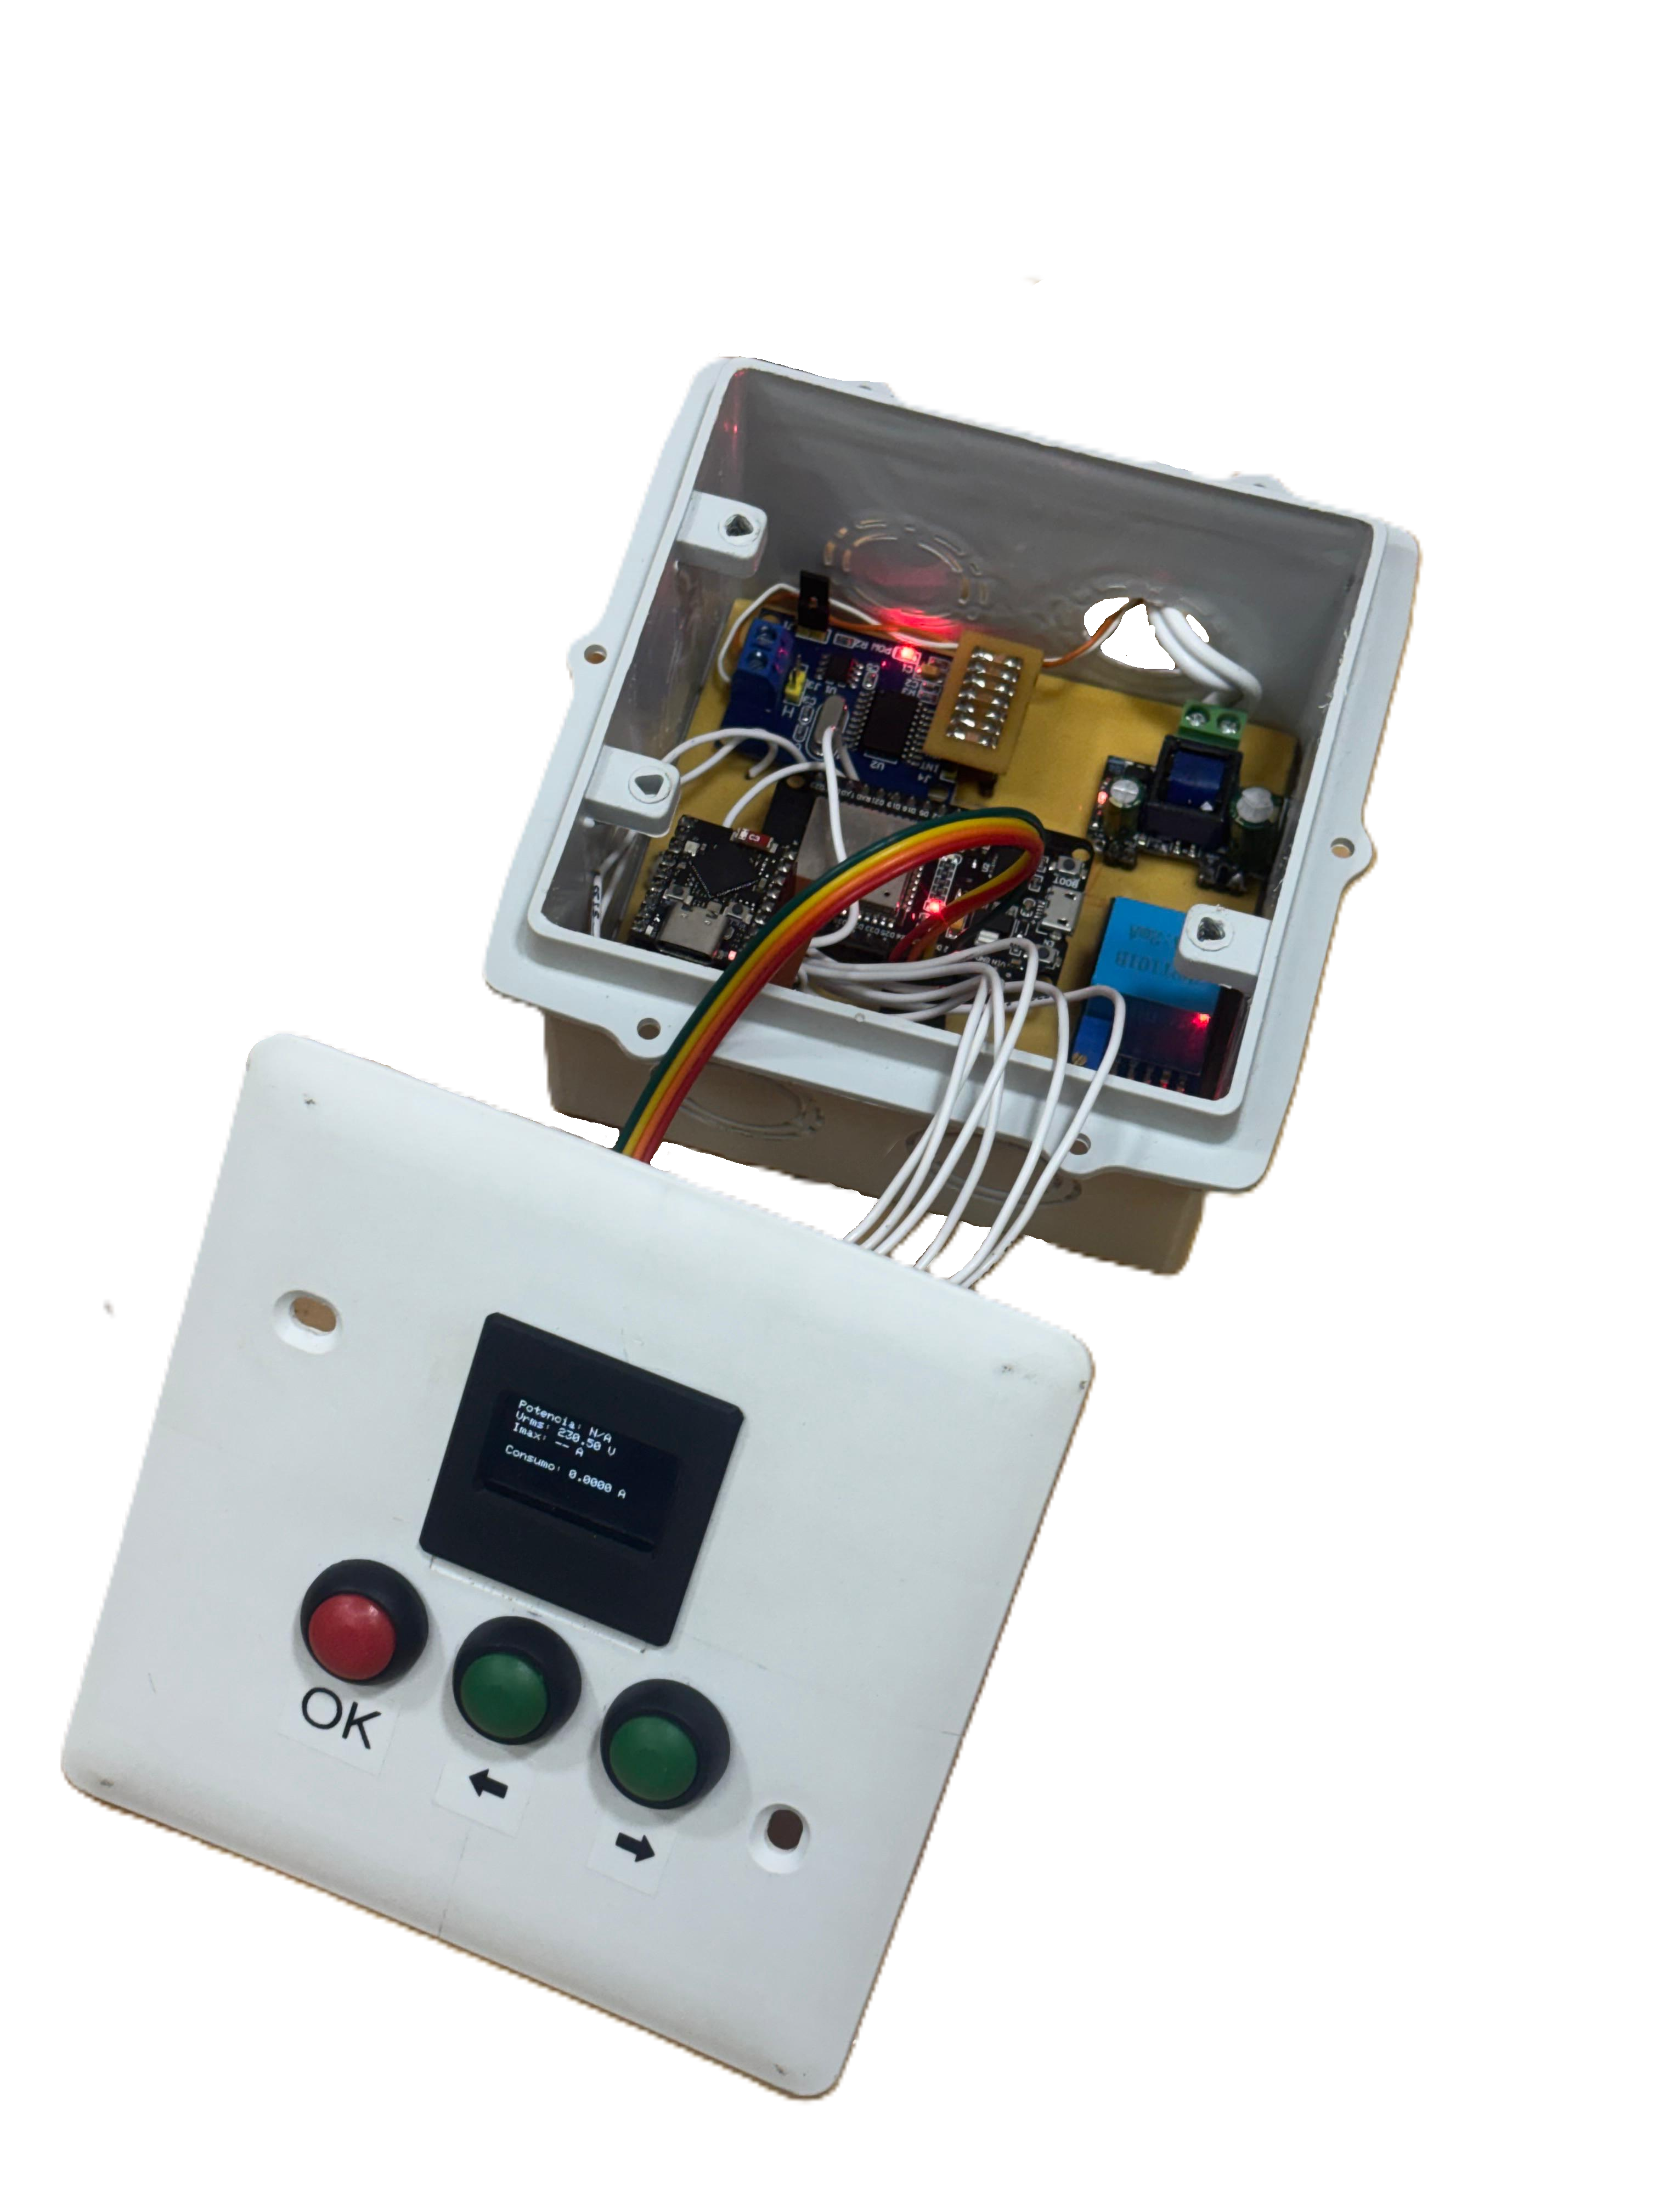
\includegraphics[width=0.35\textwidth]{imagenes/ac.png}
    \caption{Hardware desarrollado para el Agente de Carga(AC)}
    \label{img:ac}
\end{figure}
\section{Firmware}

\cleardoublepage
\chapter{Nodo de Consumo (NC)}

\section{Hardware}

Los Nodos de Consumo representan el elemento ejecutivo dentro de la arquitectura distribuida del sistema propuesto. A diferencia de los esquemas de control centralizados tradicionales, estos dispositivos brindan la capacidad de procesar información local y tomar decisiones de actuación de manera autónoma con informacion de sus pares. Para cumplir con este requisito de procesamiento distribuido, se seleccionó al igual que en el caso anterior un ESP32. Esta elección no es arbitraria; sino que responde a la necesidad de contar con un procesador de alta velocidad capaz de gestionar simultáneamente el muestreo de señales en tiempo real y el protocolo de comunicación inalámbrico ESP-NOW, todo ello manteniendo un bajo costo y un consumo energético acotado.

El desarrollo del hardware del NC enfrentó el desafío de circuitos de potencia, medición de precisión e interfaz de usuario en un volumen físico restringido. El objetivo de diseño fue lograr que el dispositivo final pudiera alojarse dentro de la cajas electricas de embutir rectangulares estándar de $5 \times 10$ cm, ya existentes en la gran mayoria de instalaciones eléctricas. Para resolver esta restricción espacial sin comprometer la seguridad ni la funcionalidad, se adoptó una estrategia de diseño modular, dividiendo el circuito en dos placas apiladas de circuito impreso (PCB).

Esta arquitectura de dos niveles cumple una doble función crítica. En primer lugar, optimiza el uso del espacio disponible dentro del gabinete. En segundo lugar, y más importante, establece una barrera de seguridad entre los circuitos de alta tensión y la lógica de control. La placa inferior está dedicada en parte al manejo de la tensión de red (220 V CA) y medicion de corriente, mientras que la placa superior aloja el microcontrolador y selector de prioridad. Esta separación física reduce significativamente el riesgo de inyectar alta tension al microcontrolador y minimiza el acoplamiento o interferencias electromagneticas provenientes de la red.

En la placa inferior, denominada etapa de potencia, se encuentran los siguientes subsistemas:
\begin{itemize}
    \item \textbf{Fuente de Alimentación:} Se integró un módulo convertidor CA-CC conmutado compacto, encargado de transformar la tensión de línea de 220 V CA a una tensión continua estable de 5 V para alimentar la lógica del sistema. La estabilidad de esta fuente es vital, ya que variaciones en la tensión de alimentación podrían introducir errores en la referencia del sensor de corriente.
    \item \textbf{Actuación:} El control de la carga se realiza mediante un relé electromecánico con capacidad de conmutación de hasta 12 A a 250 V CA. Dado que las salidas digitales del microcontrolador no poseen la capacidad de corriente suficiente para excitar directamente la bobina del relé, se implementó una etapa de potencia intermedia utilizando un transistor bipolar NPN de uso general (modelo BC337) configurado como interruptor entrando en corte y saturación.
    \item \textbf{Sensor:} La medición del consumo se realizó mediante un sensor de corriente por efecto Hall lineal ACS712. Este componente ofrece una ventaja fundamental ya que proporciona aislamiento galvánico entre el conductor de corriente (que está al potencial de red) y los pines de señal. El sensor entrega una tensión analógica proporcional a la corriente instantánea que circula hacia la carga. Sin embargo, como este módulo opera a 5 V y el ESP32 tiene entradas tolerantes solo hasta 3.3 V, fue necesario interponer un divisor de tensión resistivo para adecuar los niveles de señal y proteger al microcontrolador contra sobretensiones.
\end{itemize}

Por otra parte, la placa superior concentra las funciones de control e interacción. El módulo ESP32 se monta en esta, facilitando el acceso a sus puertos de programación y depuración. Para la configuración del dispositivo, se incorporó un interruptor tipo DIP Switch de dos vías. Este componente permite al instalador o usuario asignar una dirección de prioridad binaria (de 0 a 3) al nodo de manera física, eliminando la necesidad de conectar una computadora o dispositivo para reconfigurar el software cada vez que se cambia la función del nodo. Finalmente, para brindar retroalimentación inmediata, se diseñó primero una interfaz visual compuesta por una barra de LEDs de tres colores (rojo, amarillo y verde) que se puede observar en los Anexos ~\nameref{cap:prototipado} y ~\nameref{cap:desarrollo}. Estos indicadores permitian unicamente el estado de disponibilidad energética de la microrred. Luego como se puede ver en la Figura~\ref{fig:nc} se implemento un display OLED similar al del AC con diseño en 3D para ser adaptado a una tapa estandar de cajas rectangulares de la marca Cambre, es especifico su linea Siglo XXI.

\begin{figure}[hbt!]
    \centering
    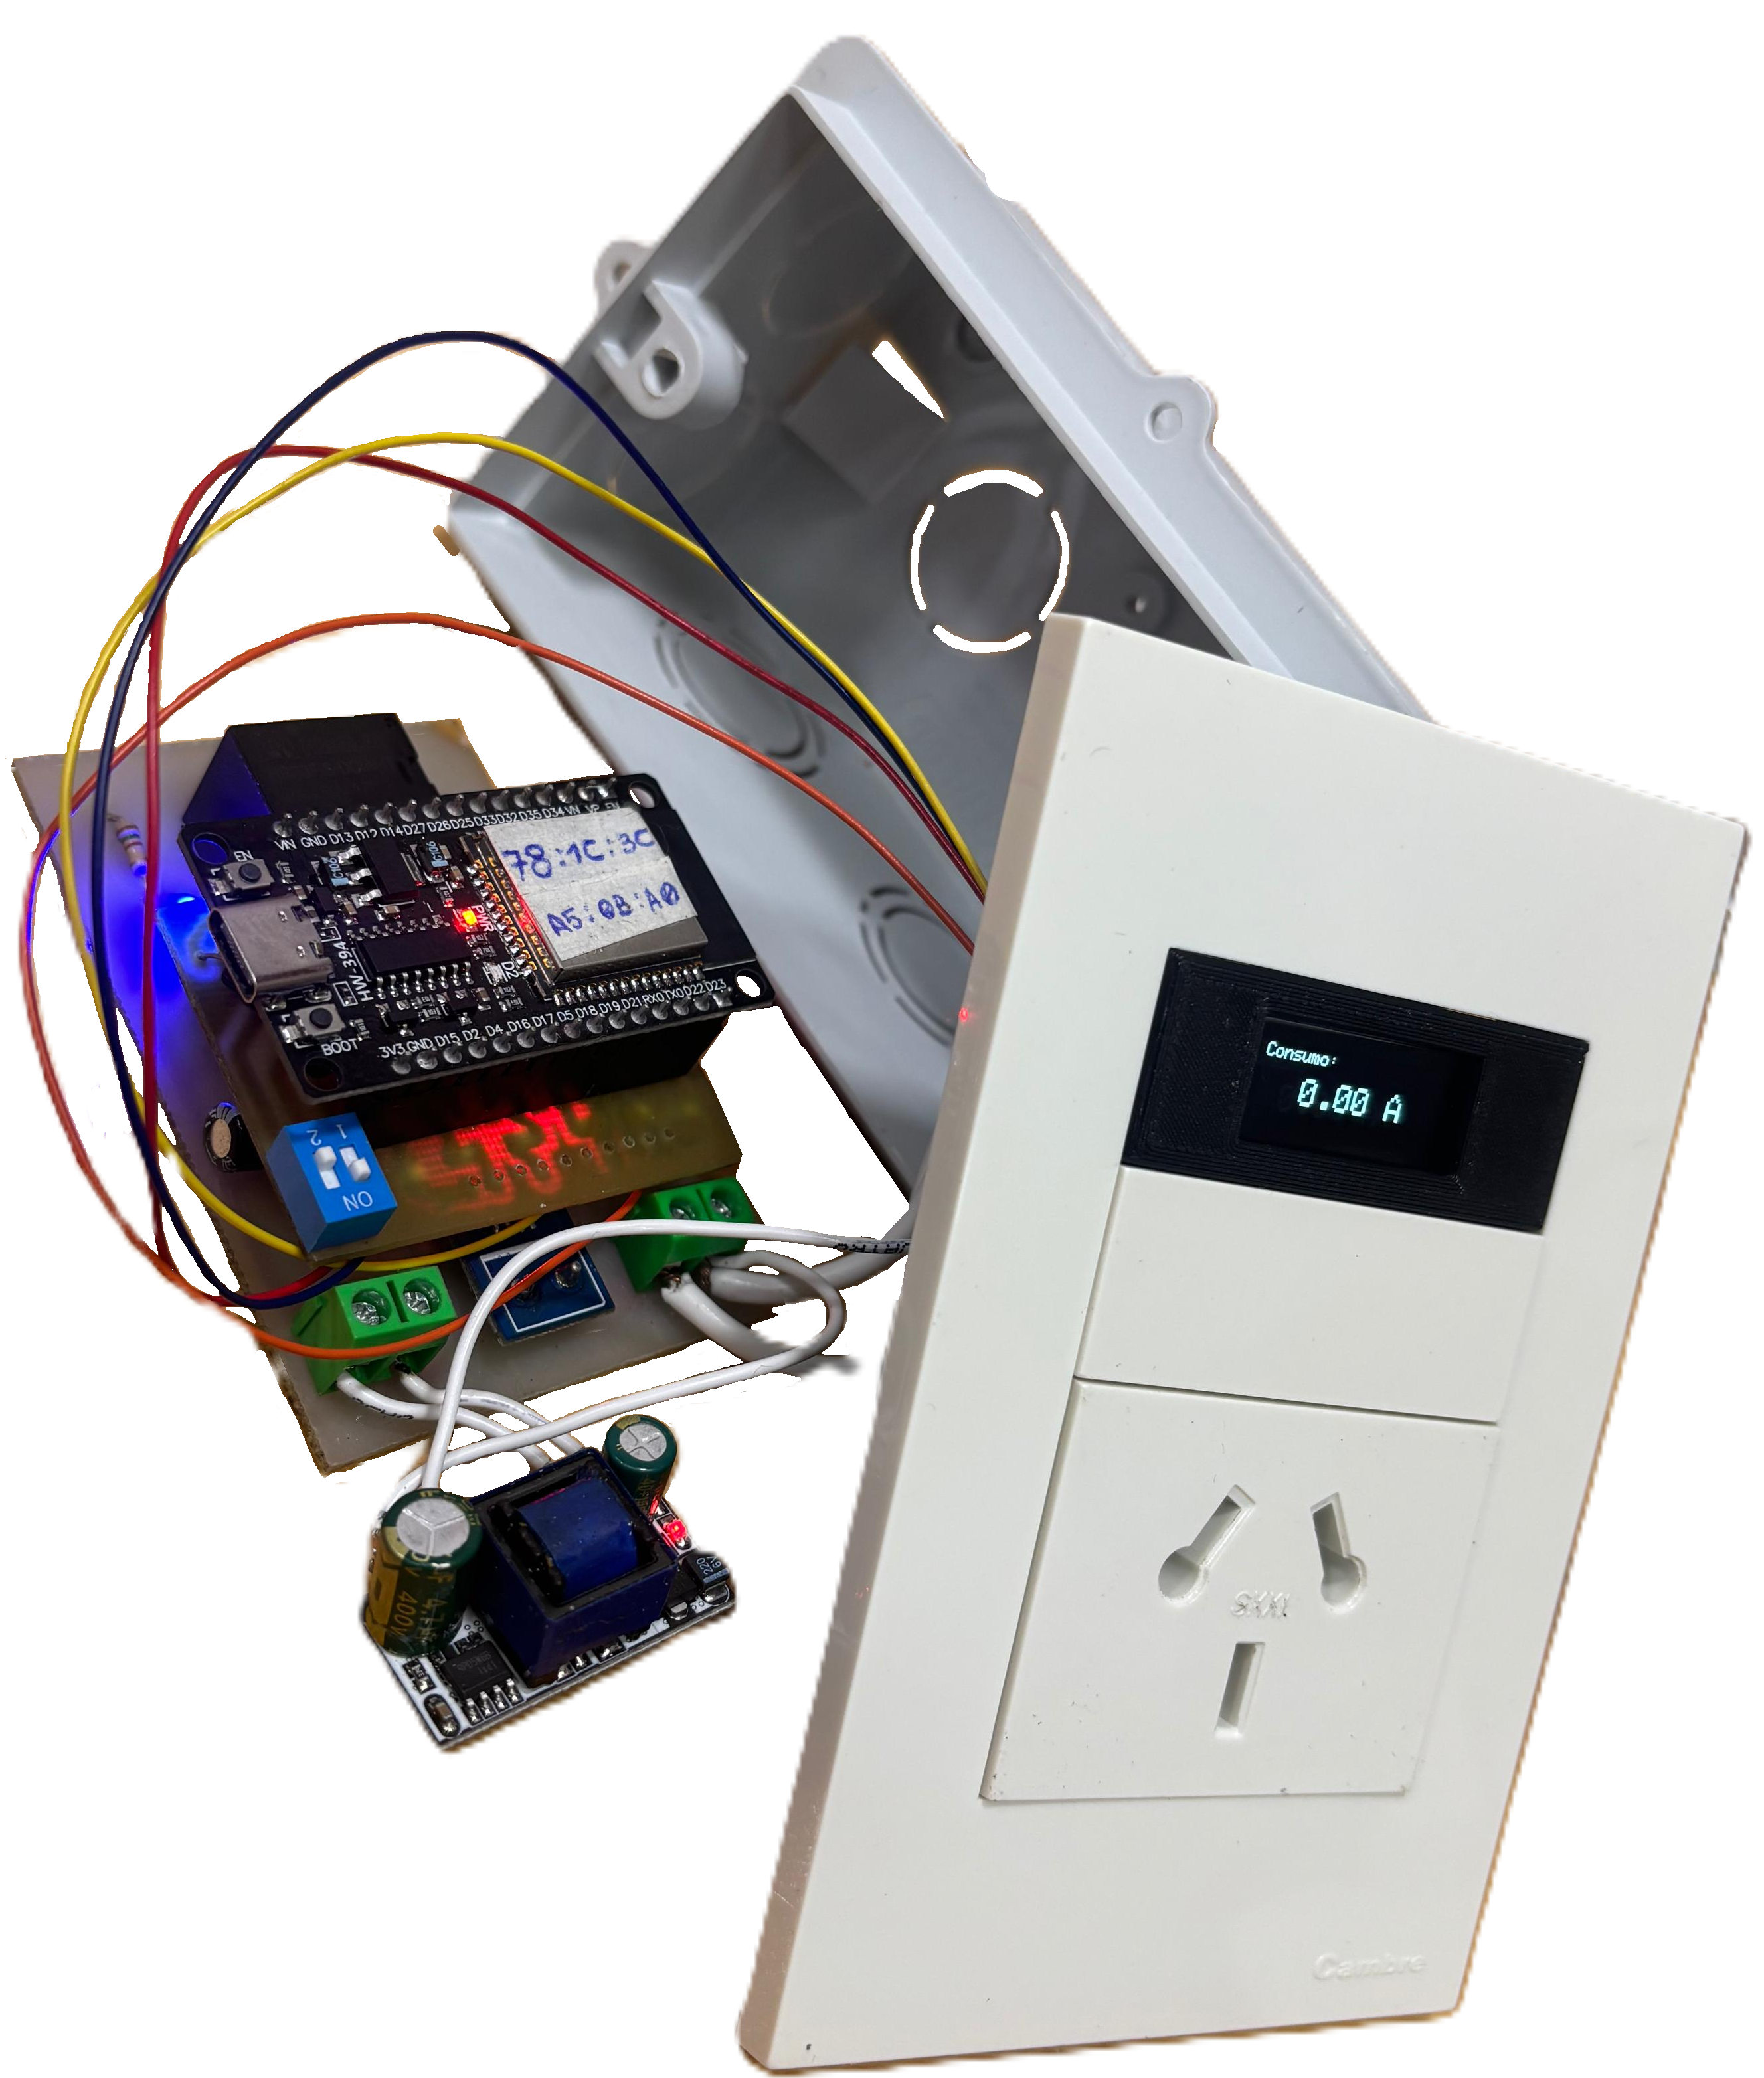
\includegraphics[width=0.6\textwidth]{imagenes/nc.jpg}
    \caption{Hardware desarrollado para el Nodo de Consumo (NC)}
    \label{fig:nc}
\end{figure}

\section{Firmware}

El firmware del NC implementa la lógica de control distribuido descrita en el Capítulo 8. Su bucle principal ejecuta tres tareas fundamentales de manera cíclica: la medición precisa del consumo, el intercambio de mensajes de consenso y la ejecución del algoritmo de decisión para la conexión o desconexión de la carga.

\subsection{Medición de Corriente}
La adquisición de la señal del sensor ACS712 sigue el mismo principio de muestreo síncrono utilizado en el AC. El microcontrolador captura la forma de onda de la corriente consumida por la carga y calcula su valor eficaz (RMS) en tiempo real.

Para validar la precisión de este método, se realizaron ensayos comparativos utilizando una punta de corriente comercial calibrada y un osciloscopio, como se muestra en la Figura~\ref{fig:prueba-corriente}. Los resultados demostraron que el sistema mantiene una linealidad adecuada y es capaz de medir correctamente incluso ante cargas no lineales (como fuentes conmutadas), reportando valores con un error en torno a los 30-40 mA siendo practicamente insignificantes respecto del valor maximo y tambien mejorable con una fuente de mayor calidad.

\begin{figure}[H]
    \centering
    \includegraphics[width=0.6\textwidth]{imagenes/prueba-corriente.jpg}
    \caption{Prueba de medición de corriente en el NC contra punta de corriente}
    \label{fig:prueba-corriente}
\end{figure}

\subsection{Lógica de Control y Actuación}
El núcleo del firmware es una máquina de estados que evalúa constantemente si la carga debe permanecer conectada o desconectada. Esta decisión se basa en la comparación entre el consumo total reportado por la red (suma de los consumos de todos los nodos) y el límite de corriente disponible informado por el AC.

\begin{itemize}
    \item \textbf{Si la carga está conectada:} El nodo verifica si el consumo total supera la disponibilidad. De ser así, y si su prioridad es la más baja de la red, procede a desconectar el relé para aliviar la carga del sistema.
    \item \textbf{Si la carga está desconectada:} El firmware aplica una lógica de reconexión con histéresis. Antes de intentar reconectar, calcula una corriente total estimada sumando el consumo actual de la red, su propio consumo histórico (guardado antes de la desconexión) y un margen de seguridad adicional. Solo si esta suma es inferior a la disponibilidad, se permite la reconexión. Esto evita oscilaciones indeseadas donde el nodo se conecta y desconecta repetidamente al estar cerca del límite.
\end{itemize}

\subsection{Interfaz de Usuario}
Para mantener al usuario informado sobre el estado operativo, el firmware gestiona un display OLED que alterna automáticamente entre diferentes vistas informativas, tal como se aprecia en la Figura~\ref{fig:pantallas}.

\begin{figure}[hbt!]
    \centering
    \subfigure[]{
        \includegraphics[width=0.2\textwidth]{imagenes/pantalla0-nc.png}
        \label{fig:pantalla0}
    }
    \hfill
    \subfigure[]{
        \includegraphics[width=0.2\textwidth]{imagenes/pantalla1-nc.png}
        \label{fig:pantalla1}
    }
    \subfigure[]{
        \includegraphics[width=0.4\textwidth]{imagenes/prioridades-nc.png}
        \label{fig:pantalla-prioridades}
    }
    \caption{Pantallas implementadas para el NC. (a) Consumo. (b) Disponibilidad. (c) Prioridades.}
    \label{fig:pantallas}
\end{figure}

\begin{itemize}
    \item \textbf{Consumo (a):} Muestra la corriente instantánea que está demandando la carga conectada al nodo.
    \item \textbf{Disponibilidad (b):} Visualiza gráficamente (mediante una barra de progreso) y numéricamente cual es la disponibilidad de la microrred.
    \item \textbf{Prioridad (c):} Indica el nivel de prioridad asignado en el hardware (Carga Crítica o No Crítica Alta, Media o Baja), permitiendo al usuario verificar la configuración del NC.
\end{itemize}
\cleardoublepage                                   
\chapter{Plataforma IoT}

\begin{figure}[hbt!]
    \centering
    \includegraphics[width=1\textwidth]{imagenes/IoT.png}
    \caption{Plataforma-IoT realizada}
    \label{img:plataforma-iot}
\end{figure}
\cleardoublepage                                   
\chapter{Integración del Sistema de Gestión de Consumos}

\begin{figure}[hbt!]
    \centering
    \includegraphics[width=0.8\textwidth]{imagenes/PFI.png}
    \caption{Integración completa del Sistema de Gestión de Consumos}
    \label{img:integracion}
\end{figure}


\begin{figure}[hbt!]
    \centering
    \includegraphics[width=0.7\textwidth]{imagenes/prueba-carga.jpg}
    \caption{Conexión de cargas para ensayo de la gestión del consumo}
    \label{img:prueba-carga}
\end{figure}

\begin{figure}[hbt!]
    \centering
    \includegraphics[width=0.7\textwidth]{imagenes/prueba.png}
    \caption{Resultados del ensayo de la gestión de consumos}
    \label{img:validacion}
\end{figure}

\part{Discusión y Conclusiones}
\cleardoublepage                                  % 
\chapter{Discusion}
\label{cap:Discusion}
 
\cleardoublepage 
\chapter{Conclusiones}
\label{cap:Conclusiones}




% \section{Comprobación final}

% Lo que sigue puede ser útil como lista de comprobación

% \subsection{Legibilidad}
% Pida siempre a otra persona que lea la tesis para comprobar su legibilidad, gramática, etc. 

% No tiene por qué ser alguien que la entienda perfectamente. De hecho, los miembros de la familia pueden ser voluntarios

\cleardoublepage 
\chapter{Trabajo a Futuro}
\label{cap:TrabajosFuturos}



% Se mantiene la numeracion de las paginas
% Pero los capitulos no se enumeran más
\backmatter 

% Anexos
%%%%%%%%%%%%%%%%%%%%%%
\appendix
\part{Anexos}
\cleardoublepage
\chapter{Circuito Esquemático del Nodo de Consumo (NC)}
\label{anx:esquematico-nc}

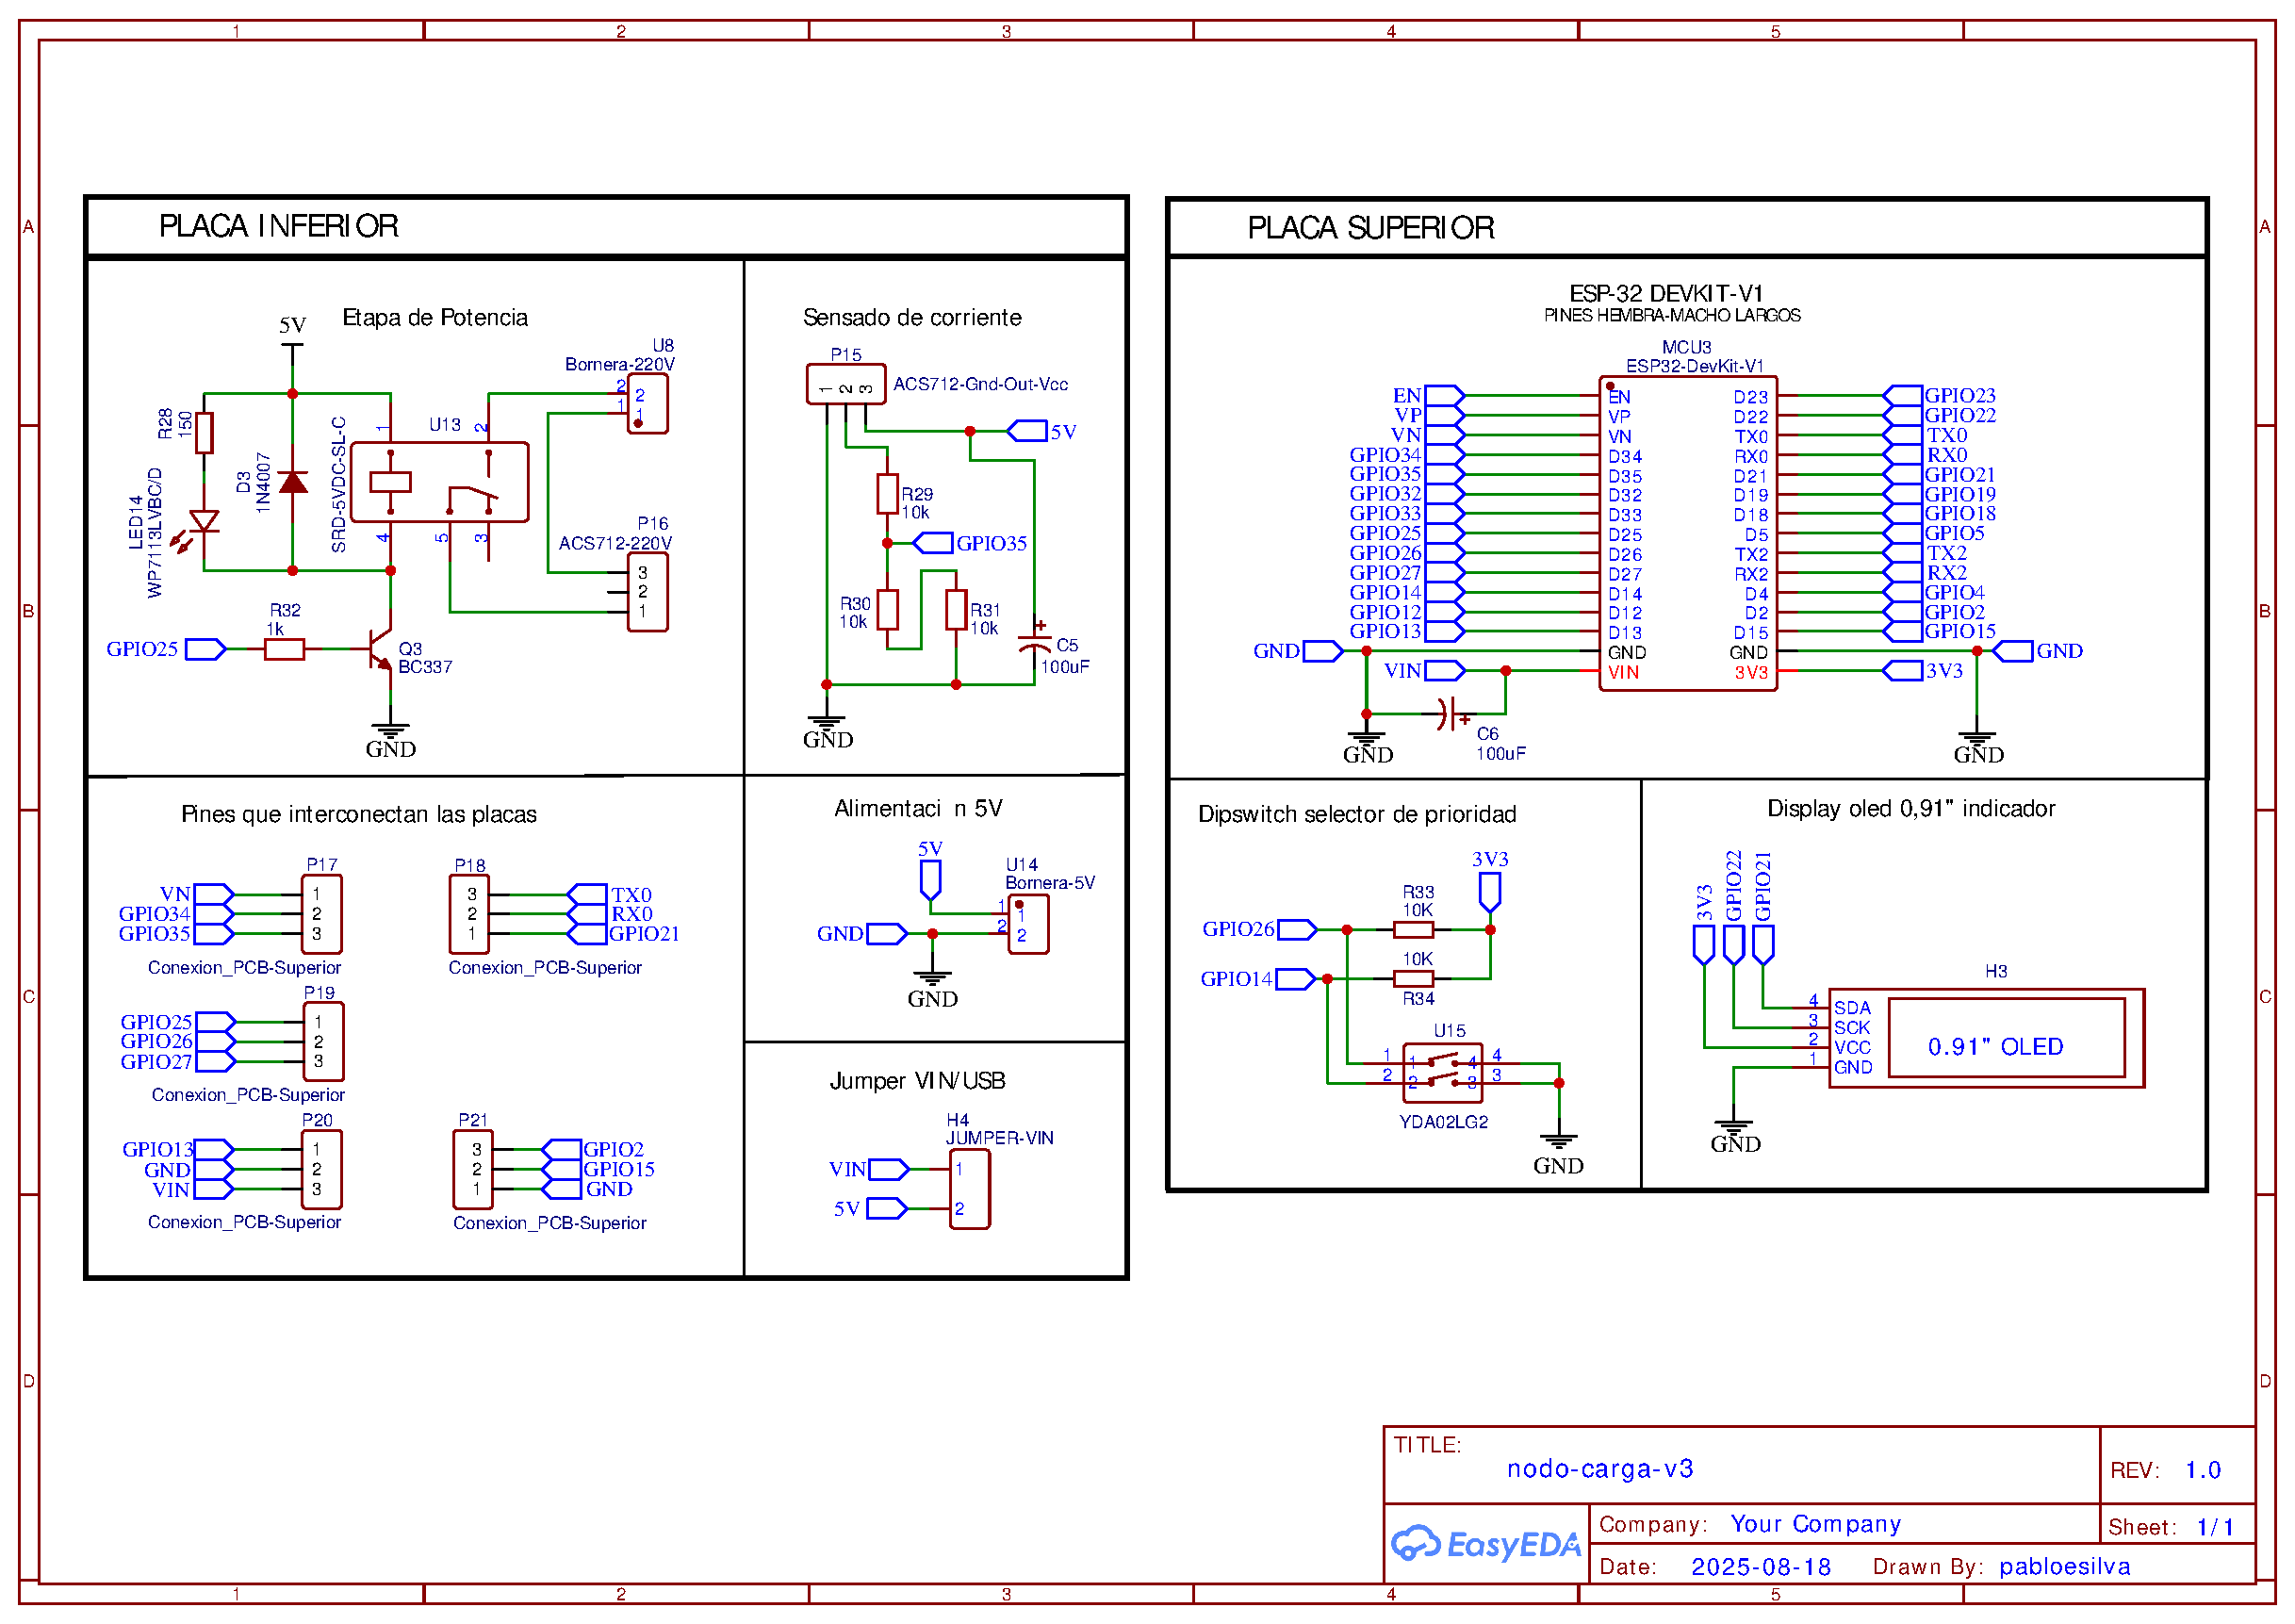
\includepdf[
    pages=-,
    scale=1,        % escalar basado en el tamaño de la página LaTeX
    fitpaper=false,  % ajusta el PDF al tamaño de la hoja
    landscape=true,
]{imagenes/esquematico-nc.pdf}



%\appendixpage
%\addappheadtotoc 
%\chapter{Población por Municipio 2010}

Municipio	Población \\
Apóstoles	29595 \\
Azara	4113 \\
San José	7095 \\
Tres Capones	1446 \\
Aristóbulo del Valle	24298 \\
Campo Grande	12676 \\
Dos de Mayo	16429 \\
Bonpland	2355 \\
Candelaria	14180 \\
Cerro Corá	1333 \\
Loreto	1113 \\
Mártires	1371 \\
Profundidad	629 \\
Santa Ana	6059 \\
Fachinal	433 \\
Garupá	46759 \\
Posadas	277564 \\
Concepción de la Sierra	7988 \\
Santa María	1589 \\
Colonia Delicia	5836 \\
Colonia Victoria	2665 \\
Eldorado	63931 \\
9 de Julio	3839 \\
Santiago de Liniers	1950 \\
Bernardo de Irigoyen	13768 \\
Comandante Andresito	19981 \\
San Antonio	9153 \\
El Soberbio	22898 \\
San Vicente	44999 \\
Colonia Wanda	15529 \\
Puerto Esperanza	17155 \\
Puerto Iguazú	42849 \\
Puerto Libertad	6694 \\
Almafuerte	1016 \\
Arroyo del Medio	2156 \\
Caa Yarí	822 \\
Cerro Azul	5854 \\
Dos Arroyos	2894 \\
Gobernador López	2283 \\
Leandro N. Alem	28583 \\
Olegario Víctor Andrade	1467 \\
Capioví	6097 \\
El Alcázar	5297 \\
Garuhapé	9355 \\
Puerto Leoni	2677 \\
Puerto Rico	19500 \\
Ruiz de Montoya	3635 \\
Caraguatay	3378 \\
Montecarlo	24338 \\
Puerto Piray	9029 \\
Campo Ramón	10070 \\
Campo Viera	10078 \\
Colonia Alberdi	3751 \\
General Alvear	1260 \\
Guaraní	4857 \\
Los Helechos	3315 \\
Oberá	66112 \\
Panambí	5928 \\
San Martín	2130 \\
Colonia Polana	935 \\
Corpus	3568 \\
General Urquiza	1216 \\
Gobernador Roca	6668 \\
Hipólito Yrigoyen	2296 \\
Jardín América	25726 \\
San Ignacio	11210 \\
Santo Pipó	6109 \\
Florentino Ameghino	2227 \\
Itacaruaré	3398 \\
Mojón Grande	2251 \\
San Javier	13030 \\
San Pedro	31051 \\
Alba Posse	7098 \\
Colonia Aurora	7744 \\
25 de Mayo	12912 \\
 %% Esto es solo un ejemplo

% Abreviaturas
%%%%%%%%%%%%%%%%%%%%%%
\clearpage
\printglossary[type=\acronymtype,title={Acrónimos}]

% Glosario de términos
%%%%%%%%%%%%%%%%%%%%%%
\glsaddall
\printglossary[type=main,title={Glosario de Términos}]
%\printnoidxglossary[type=main,sort=word,title={Glosario de Términos}]

\part{Referencias}
% Bibiografia por tipo
%%%%%%%%%%%%%%%%%%%%%%%%%
%\cleardoublepage
%\chapter{Bibliografía}
\printbibliography[]

\end{document}

